


\subsection{Exercício 3: Construção e Exploração do Conjunto de Mandelbrot}


\begin{enumerate}
  \item[(a)] Ao alterar o raio de convergência e o número de iterações no código, o que acontece com a velocidade de processamento, o detalhamento e a precisão da imagem? Para isso, teste valores no código e analise a diferença
  no resultado.

\textbf{\color{red} Falta a parte do raio de convergência}

\begin{figure}[H]
    \centering
    \subfloat[10 iterações]{
            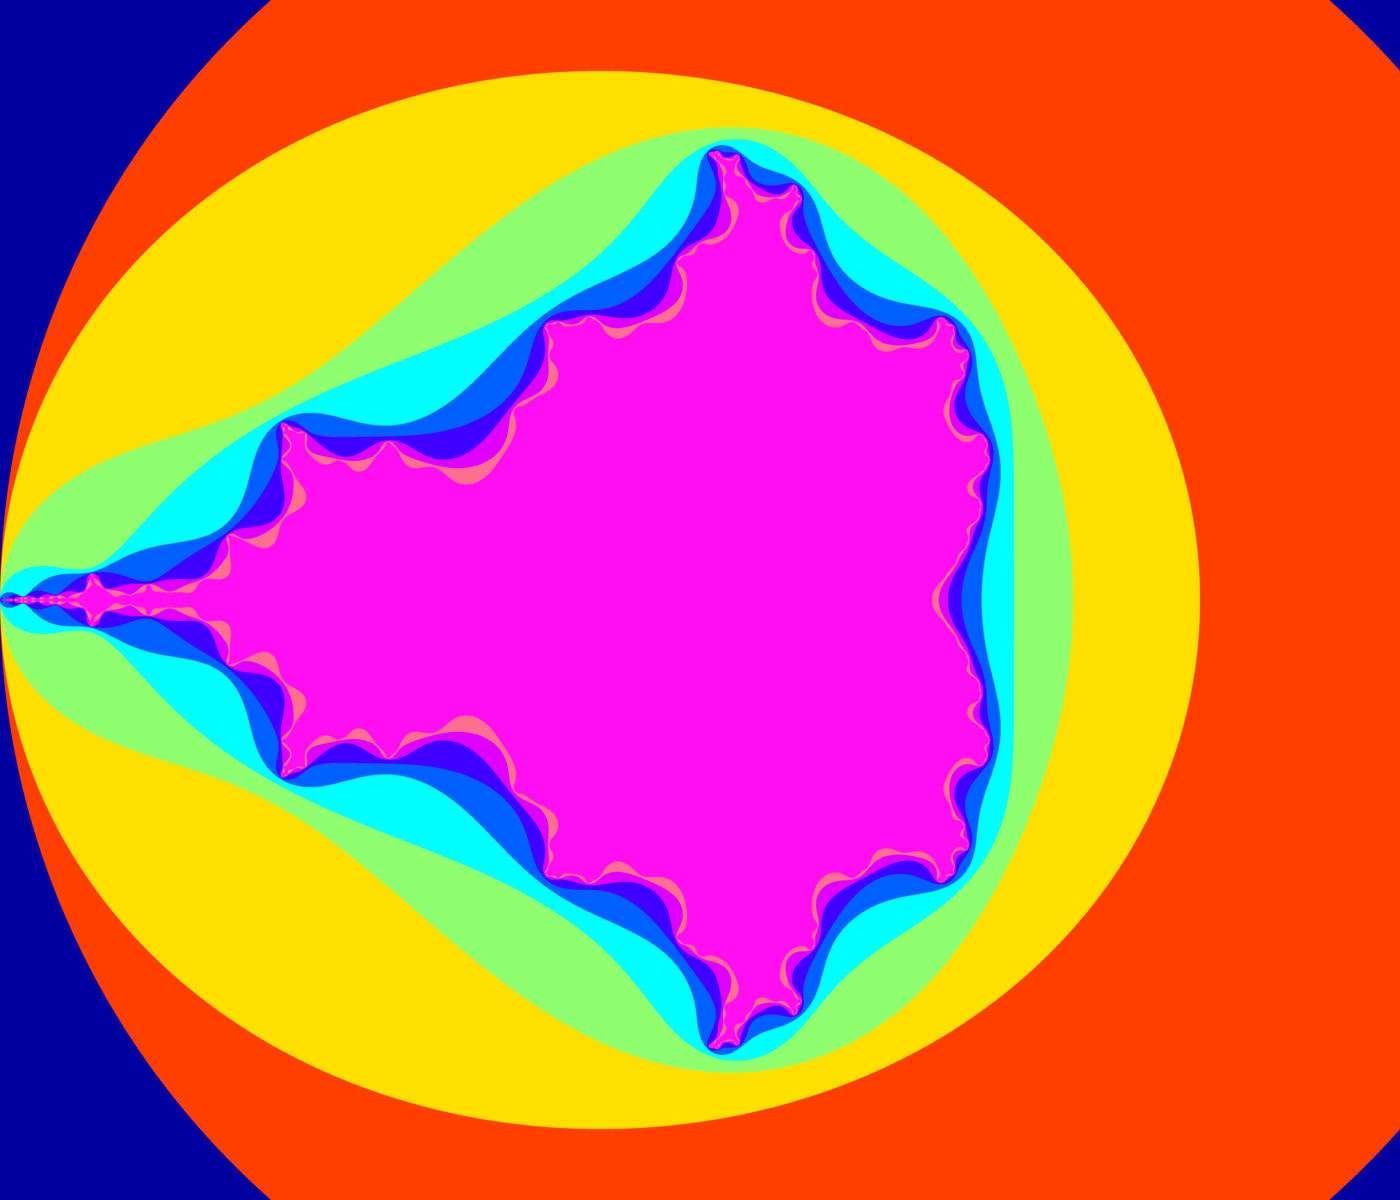
\includegraphics[width=0.3\textwidth]{figures/mandelbrot/exponent-2/mandelbrot-10-iterations-z0(0.000000,0.000000).png}
    }
    \subfloat[20 iterações]{
            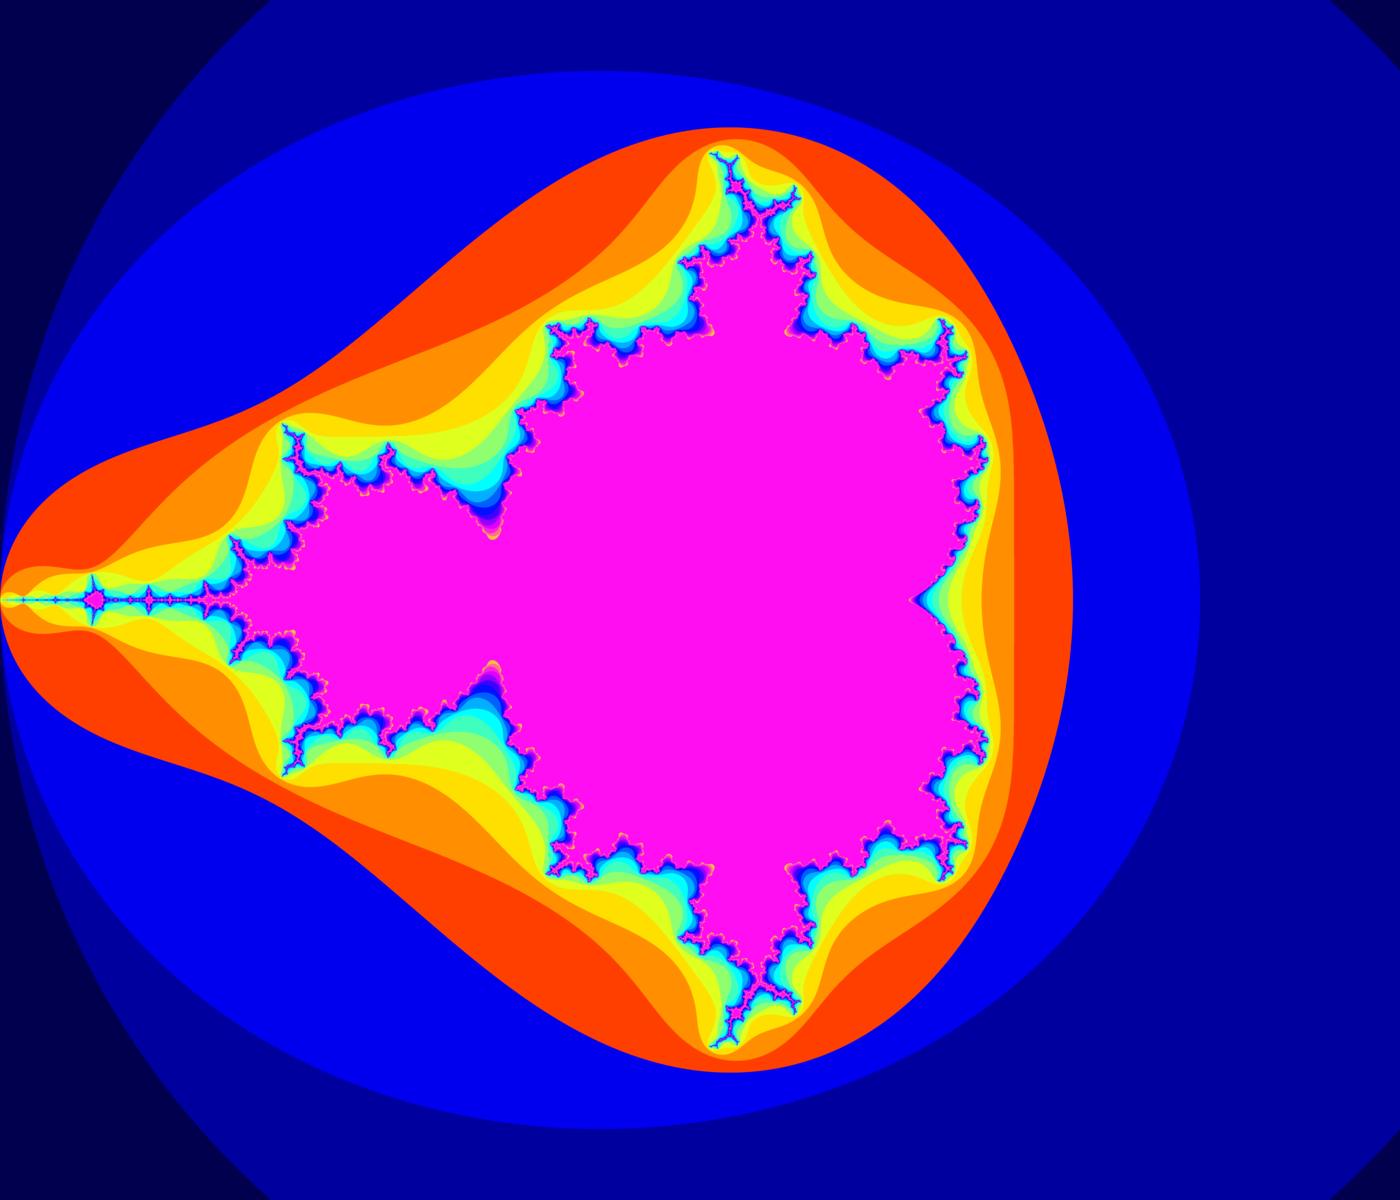
\includegraphics[width=0.3\textwidth]{figures/mandelbrot/exponent-2/mandelbrot-20-iterations-z0(0.000000,0.000000).png}
    }
    \subfloat[35 iterações]{
            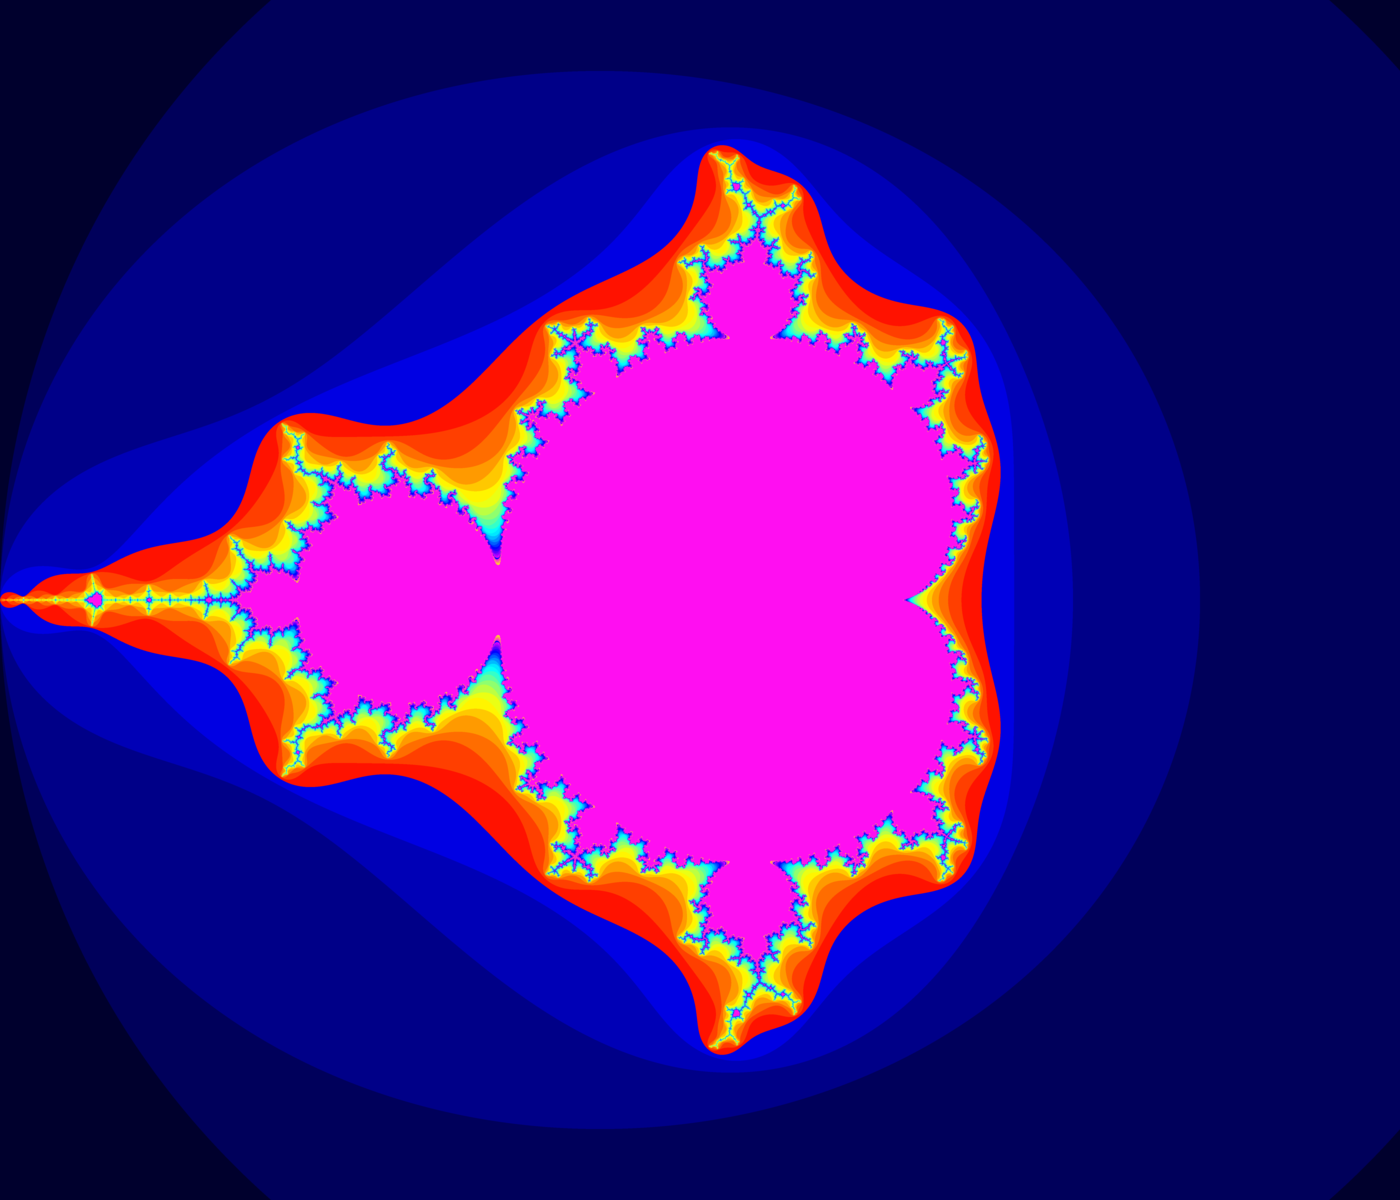
\includegraphics[width=0.3\textwidth]{figures/mandelbrot/exponent-2/mandelbrot-35-iterations-z0(0.000000,0.000000).png}
    }
    \\
    \subfloat[50 iterações]{
            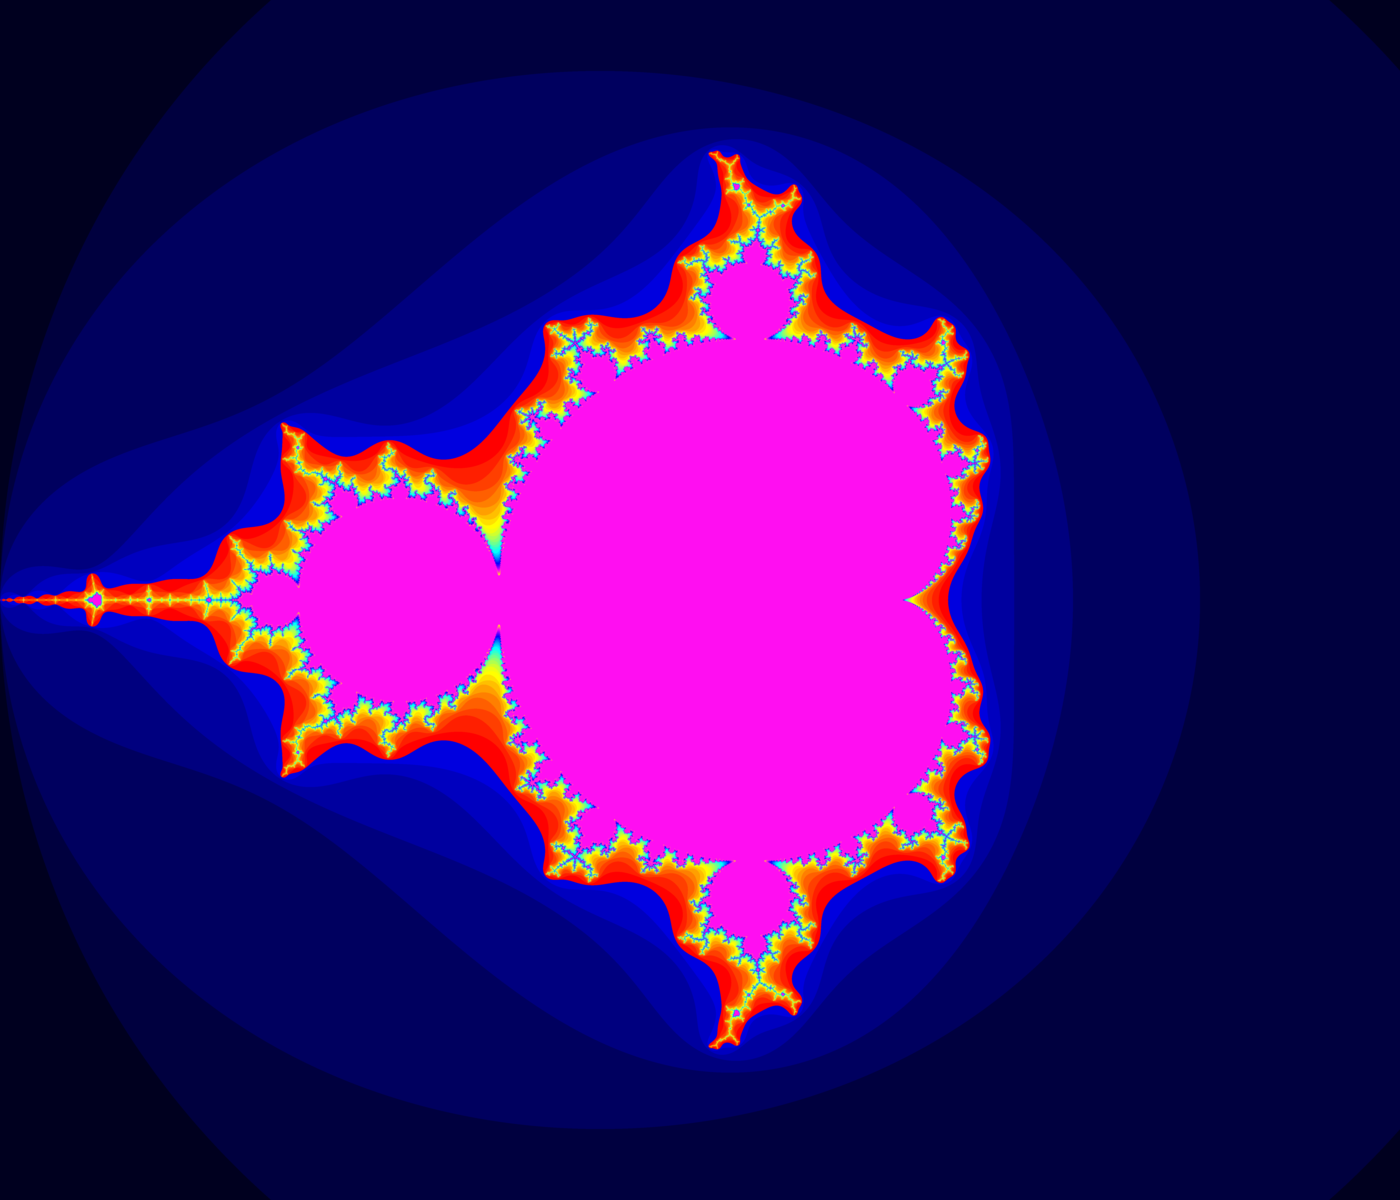
\includegraphics[width=0.3\textwidth]{figures/mandelbrot/exponent-2/mandelbrot-50-iterations-z0(0.000000,0.000000).png}
    }
    \subfloat[70 iterações]{
            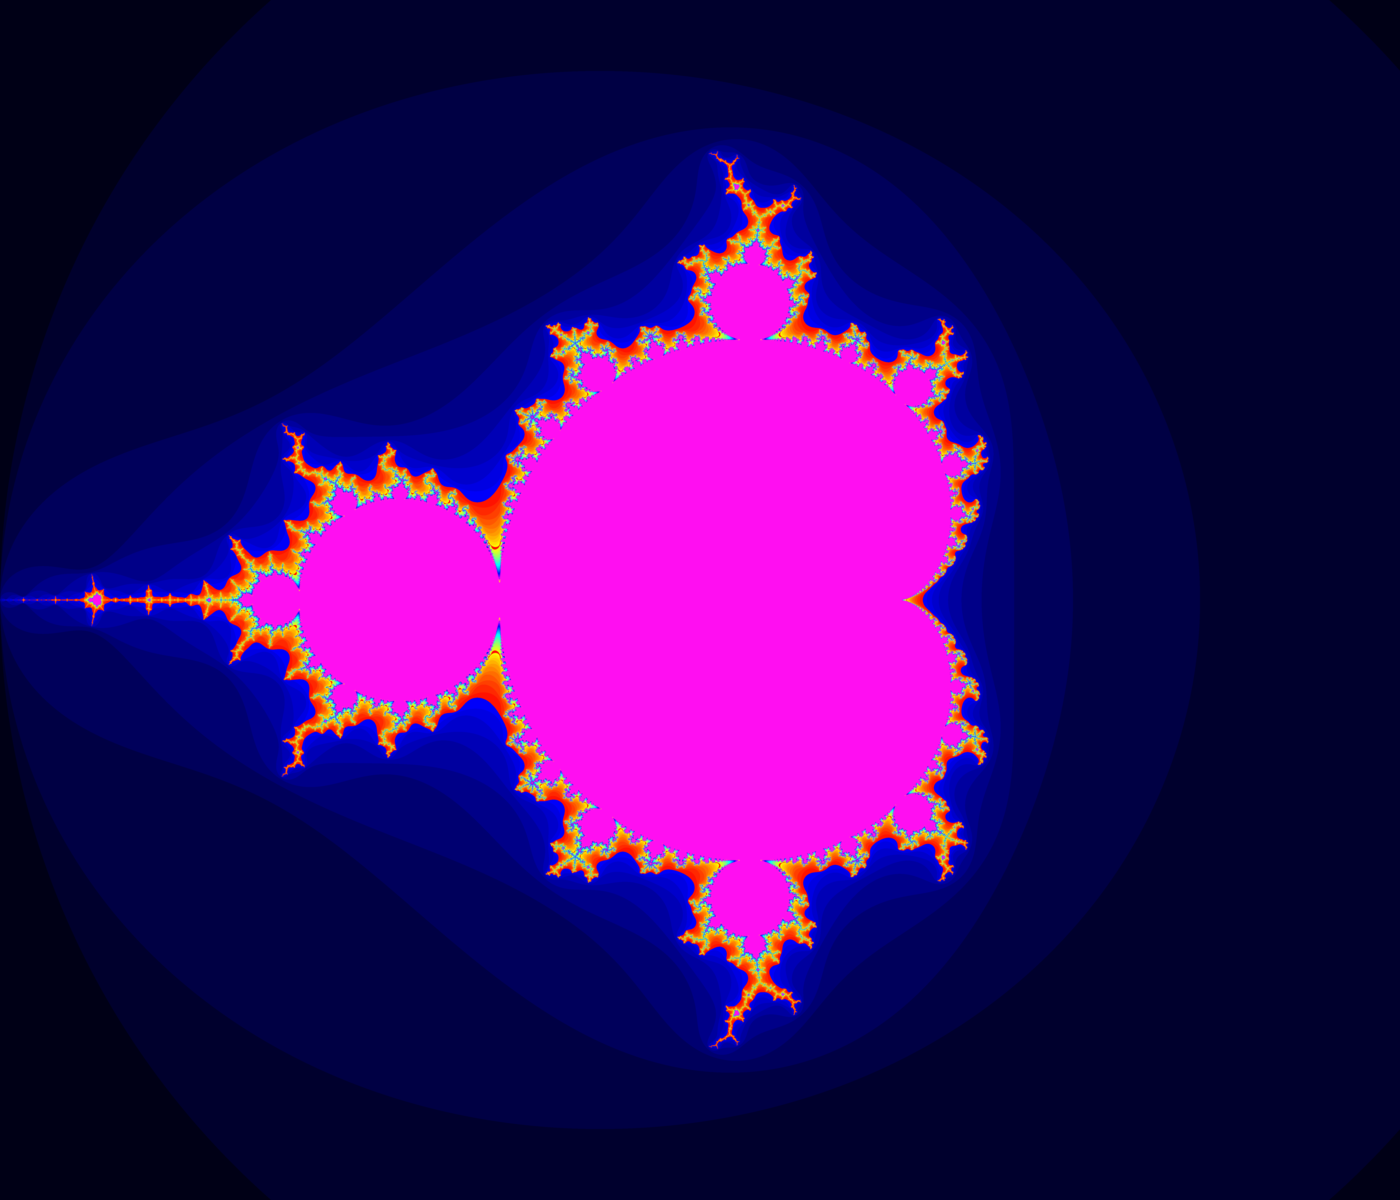
\includegraphics[width=0.3\textwidth]{figures/mandelbrot/exponent-2/mandelbrot-70-iterations-z0(0.000000,0.000000).png}
    }
    \subfloat[125 iterações]{
            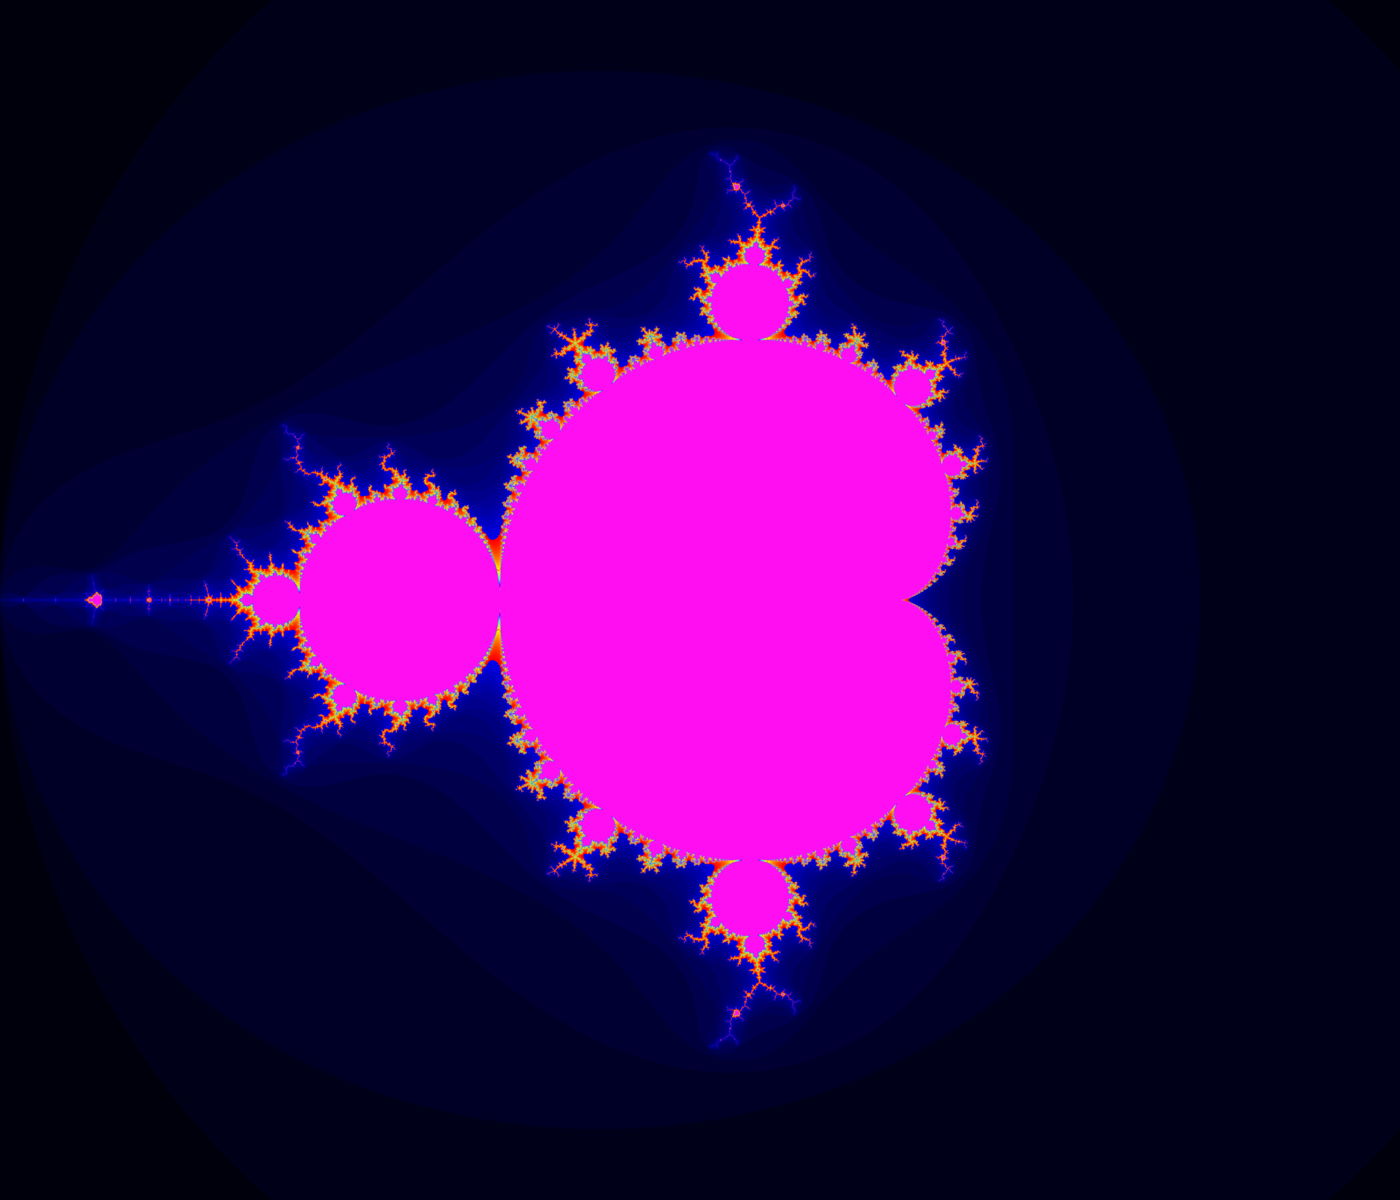
\includegraphics[width=0.3\textwidth]{figures/mandelbrot/exponent-2/mandelbrot-125-iterations-z0(0.000000,0.000000).png}
    }
    \\
    \subfloat[250 iterações]{
            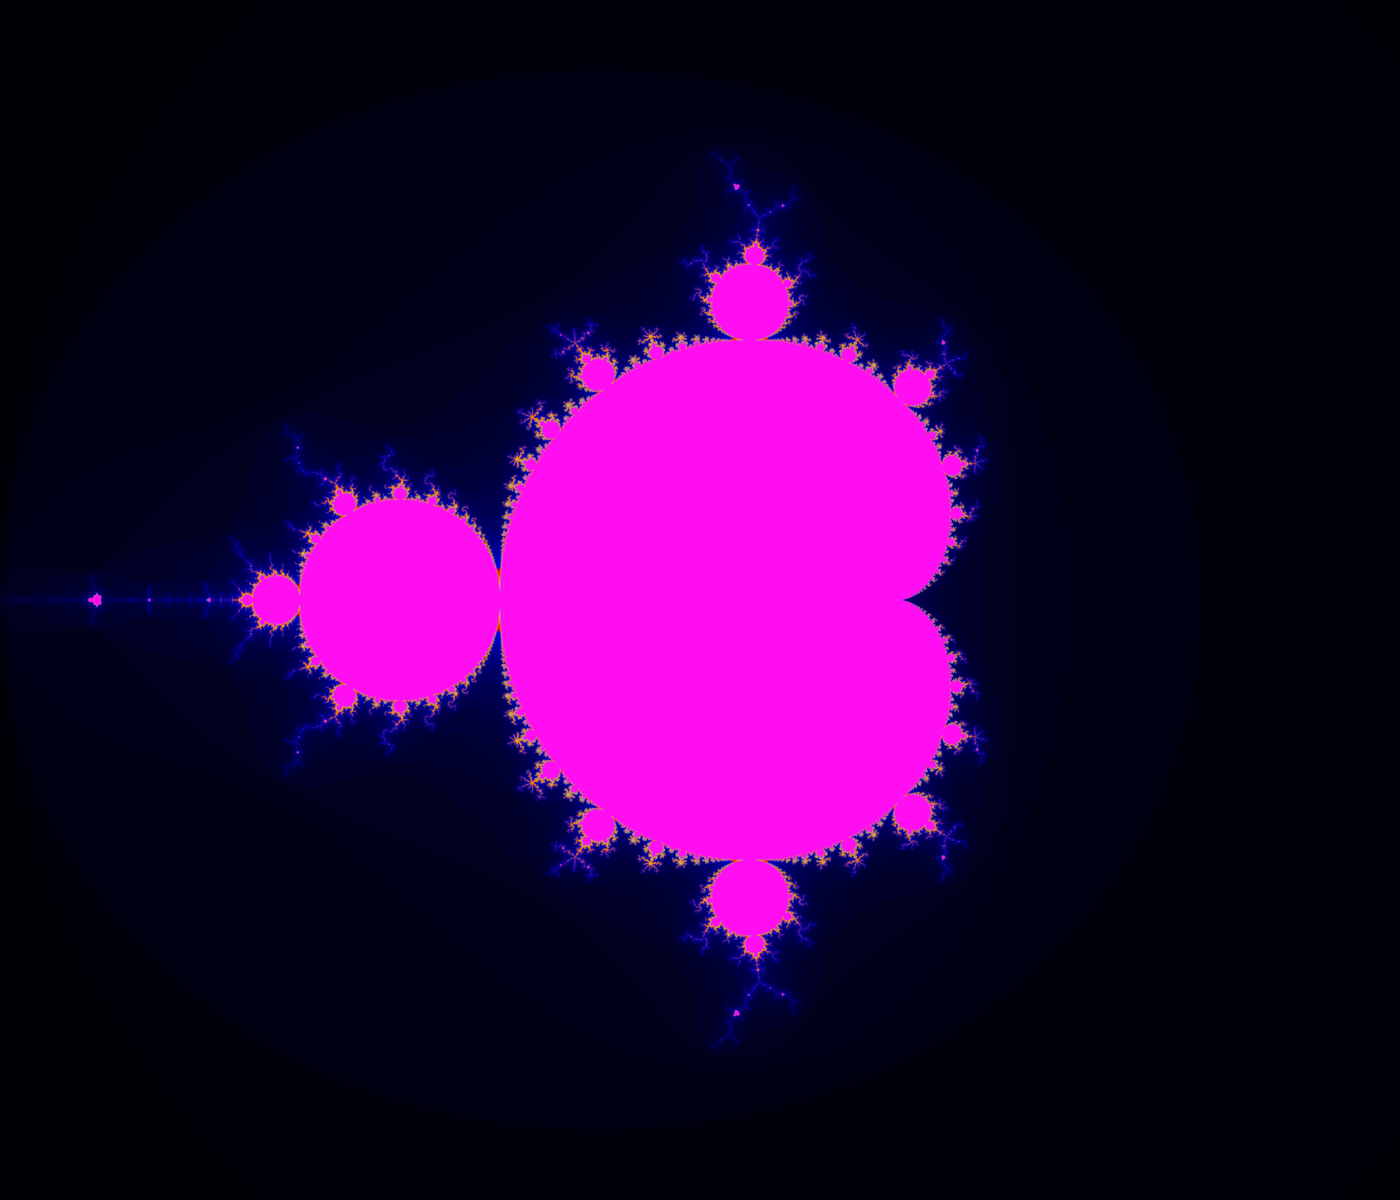
\includegraphics[width=0.3\textwidth]{figures/mandelbrot/exponent-2/mandelbrot-250-iterations-z0(0.000000,0.000000).png}
    }
    \subfloat[500 iterações]{
            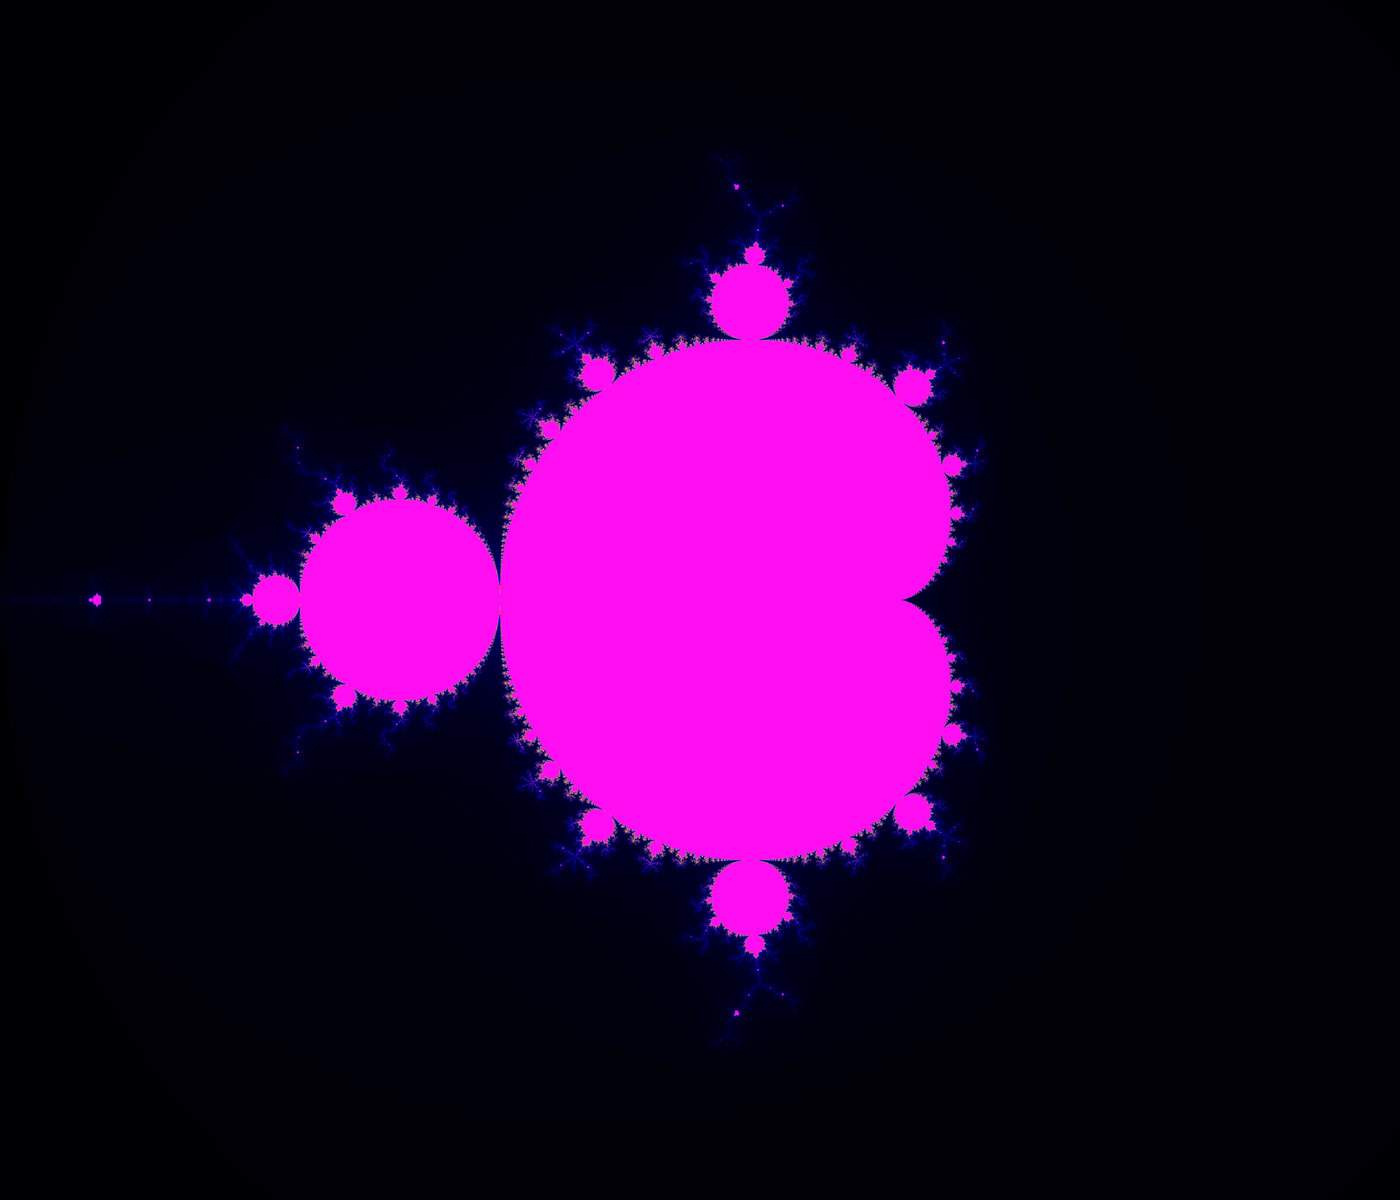
\includegraphics[width=0.3\textwidth]{figures/mandelbrot/exponent-2/mandelbrot-500-iterations-z0(0.000000,0.000000).png}
    }
    \subfloat[2000 iterações]{
            
\includegraphics[width=0.3\textwidth]{figures/mandelbrot/exponent-2/mandelbrot-2000-iterations-z0(0.000000,0.000000).png}
    }
    \caption{Conjuntos de Mandelbrot para diferentes números de iterações. Cada subfigura apresenta o conjunto gerado para o respectivo número de iterações.}
\end{figure} 

    As cores das imagens geradas representam a taxa de divergência dos números complexos no plano. Cada cor indica o número de iterações necessárias para que o valor escape para o infinito, ou seja, para que o módulo do número complexo ultrapasse o raio de convergência definido. Abaixo está a interpretação das cores:

    \begin{itemize}
        \item \textbf{Azul}: Representa os pontos que divergem rapidamente, escapando para o infinito em poucas iterações.
        \item \textbf{Verde}: Indica pontos que levam um número moderado de iterações para divergir.
        \item \textbf{Amarelo e Laranja}: Representam pontos que estão próximos à fronteira do conjunto de Mandelbrot, levando mais iterações para divergir.
        \item \textbf{Vermelho}: Indica pontos que estão ainda mais próximos da fronteira, divergindo muito lentamente.
        \item \textbf{Rosa}: Representa os pontos que não divergem, ou seja, pertencem ao conjunto de Mandelbrot.
    \end{itemize}

    Essa paleta de cores ajuda a visualizar a complexidade e os detalhes do conjunto de Mandelbrot, destacando as regiões de transição entre os pontos que pertencem ao conjunto e os que não pertencem.

    Ao alterar o número de iterações, conseguimos identificar com maior precisão os números complexos que divergem. Um número maior de iterações permite capturar mais detalhes do conjunto de Mandelbrot, evidenciando regiões de transição entre os pontos que pertencem ao conjunto e os que não pertencem. No entanto, isso também aumenta o tempo de processamento, pois mais cálculos são necessários para determinar a convergência ou divergência de cada ponto.


  \item[(b)] A Outros fractais podem ser gerados a partir do Mandelbrot, uma família de exemplos é obtida ao alterar a condição inicial $z_0 = 0$ para outros valores. Gere alguns exemplos desses conjuntos.

\begin{figure}[H]
    \centering
    \subfloat[$z_0 = (0.30, 0.10)$]{
        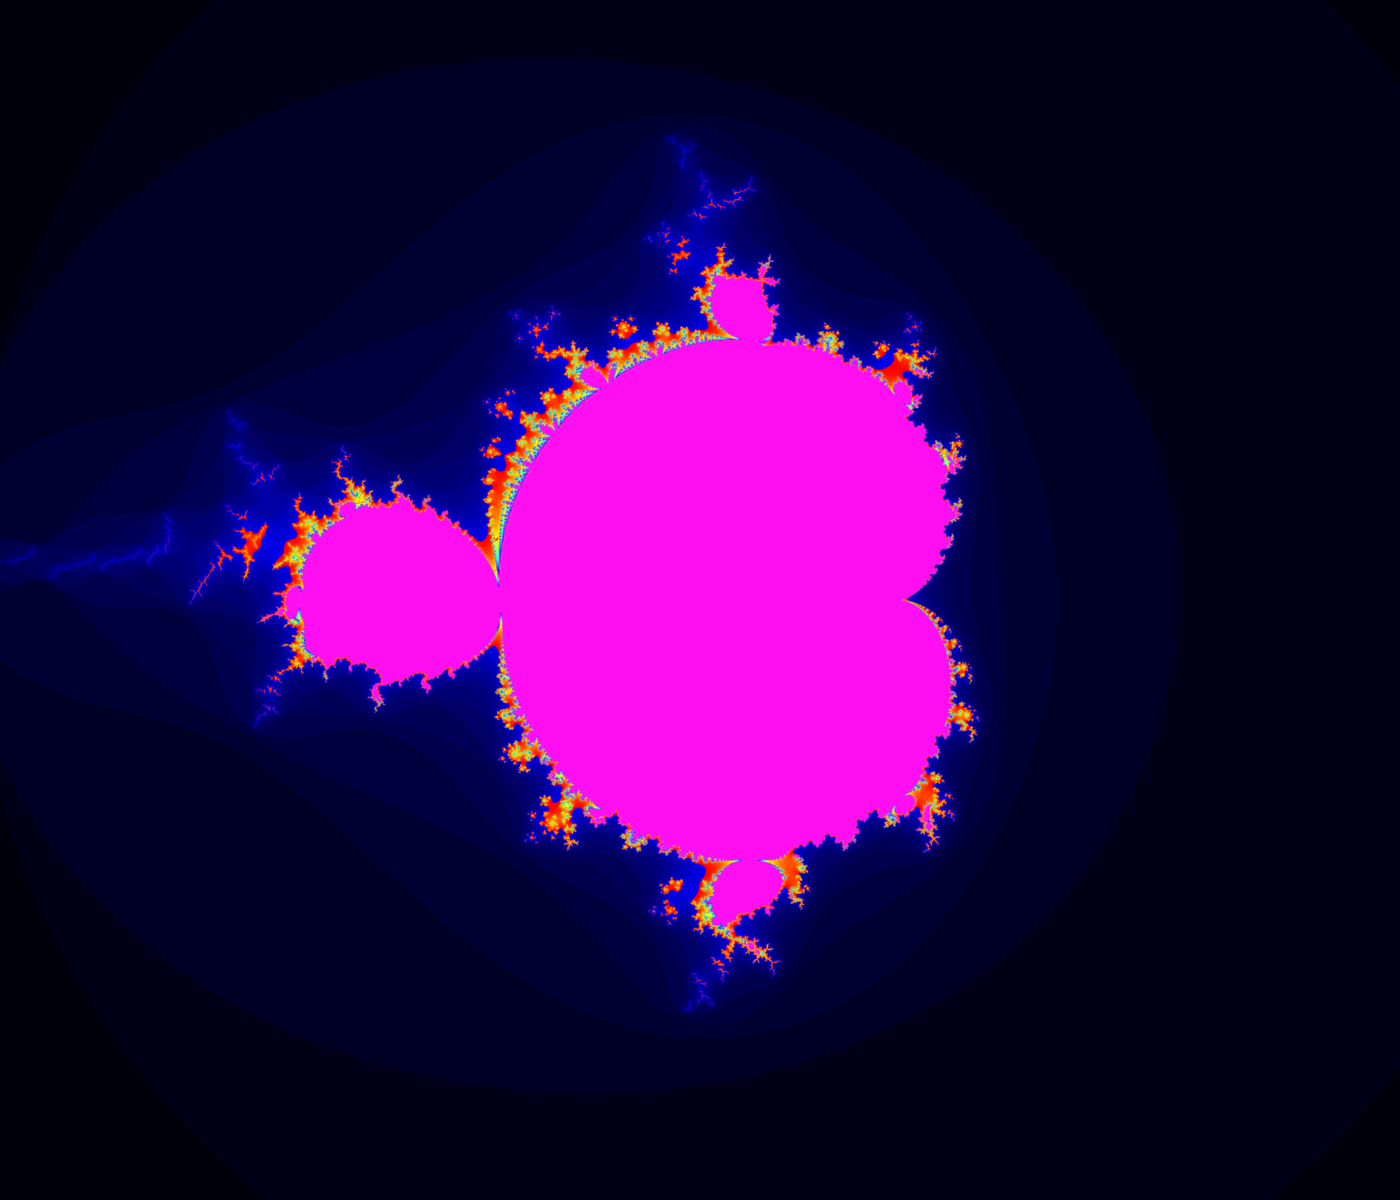
\includegraphics[width=0.3\textwidth]{figures/mandelbrot/exponent-2/mandelbrot-125-iterations-z0(0.300000,0.100000).png}
    }
    \subfloat[$z_0 = (0.30, 0.50)$]{
        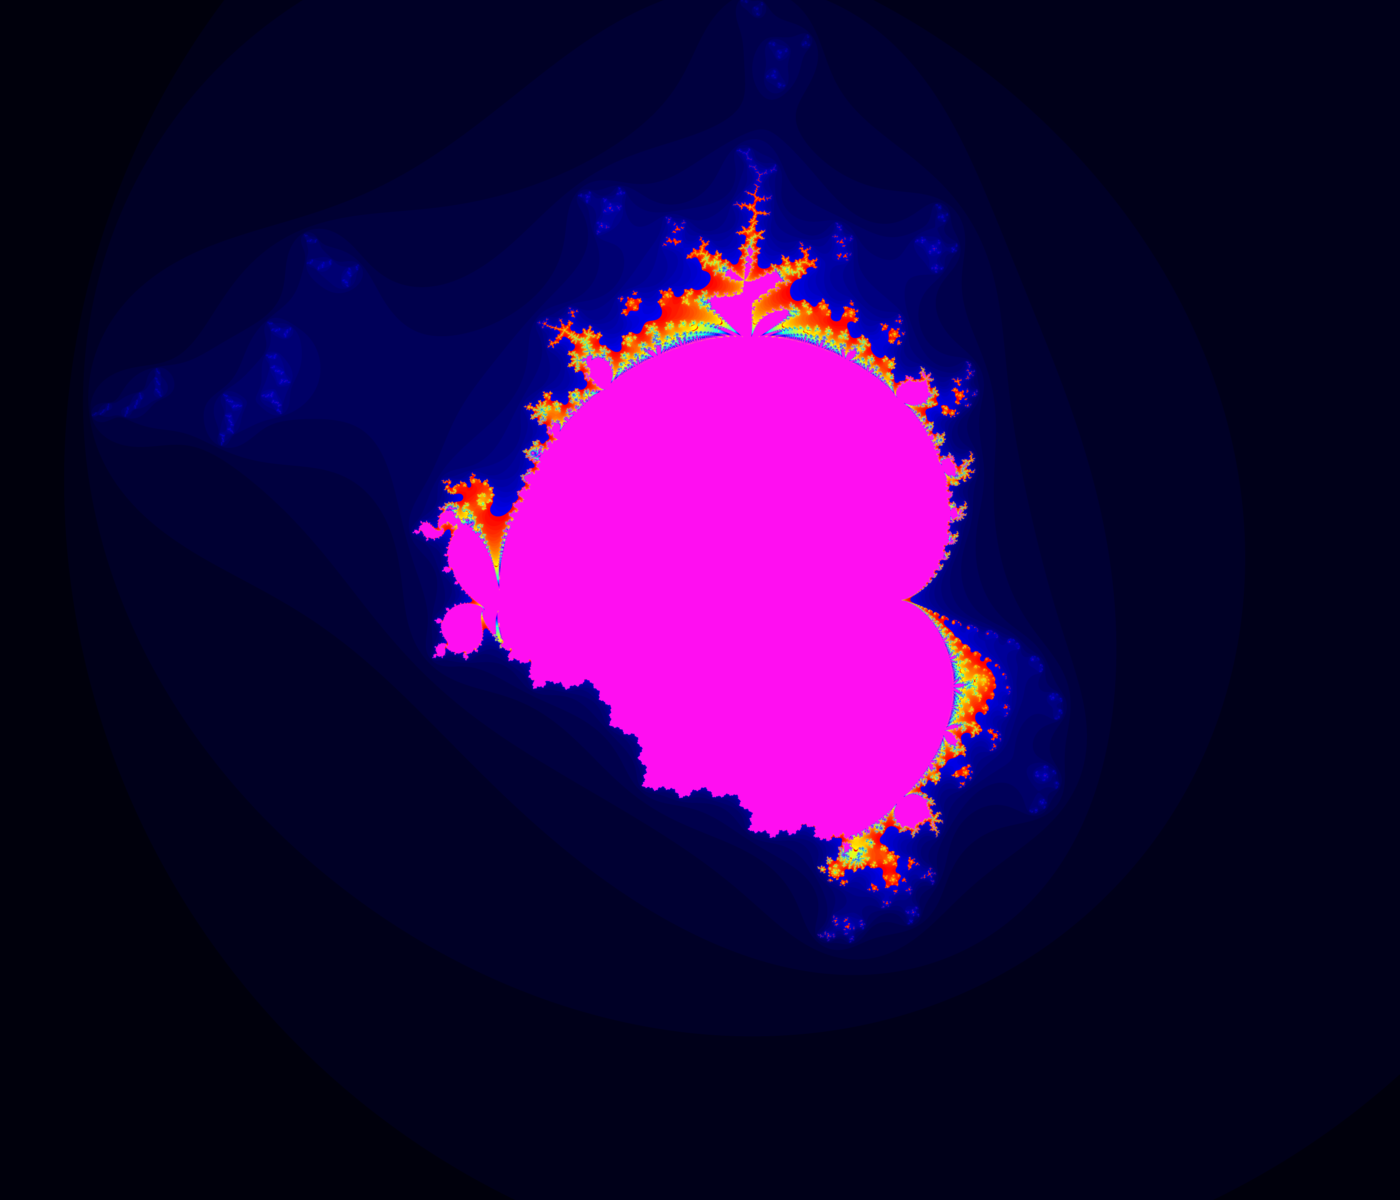
\includegraphics[width=0.3\textwidth]{figures/mandelbrot/exponent-2/mandelbrot-125-iterations-z0(0.300000,0.500000).png}
    }
    \subfloat[$z_0 = (0.50, 0.50)$]{
        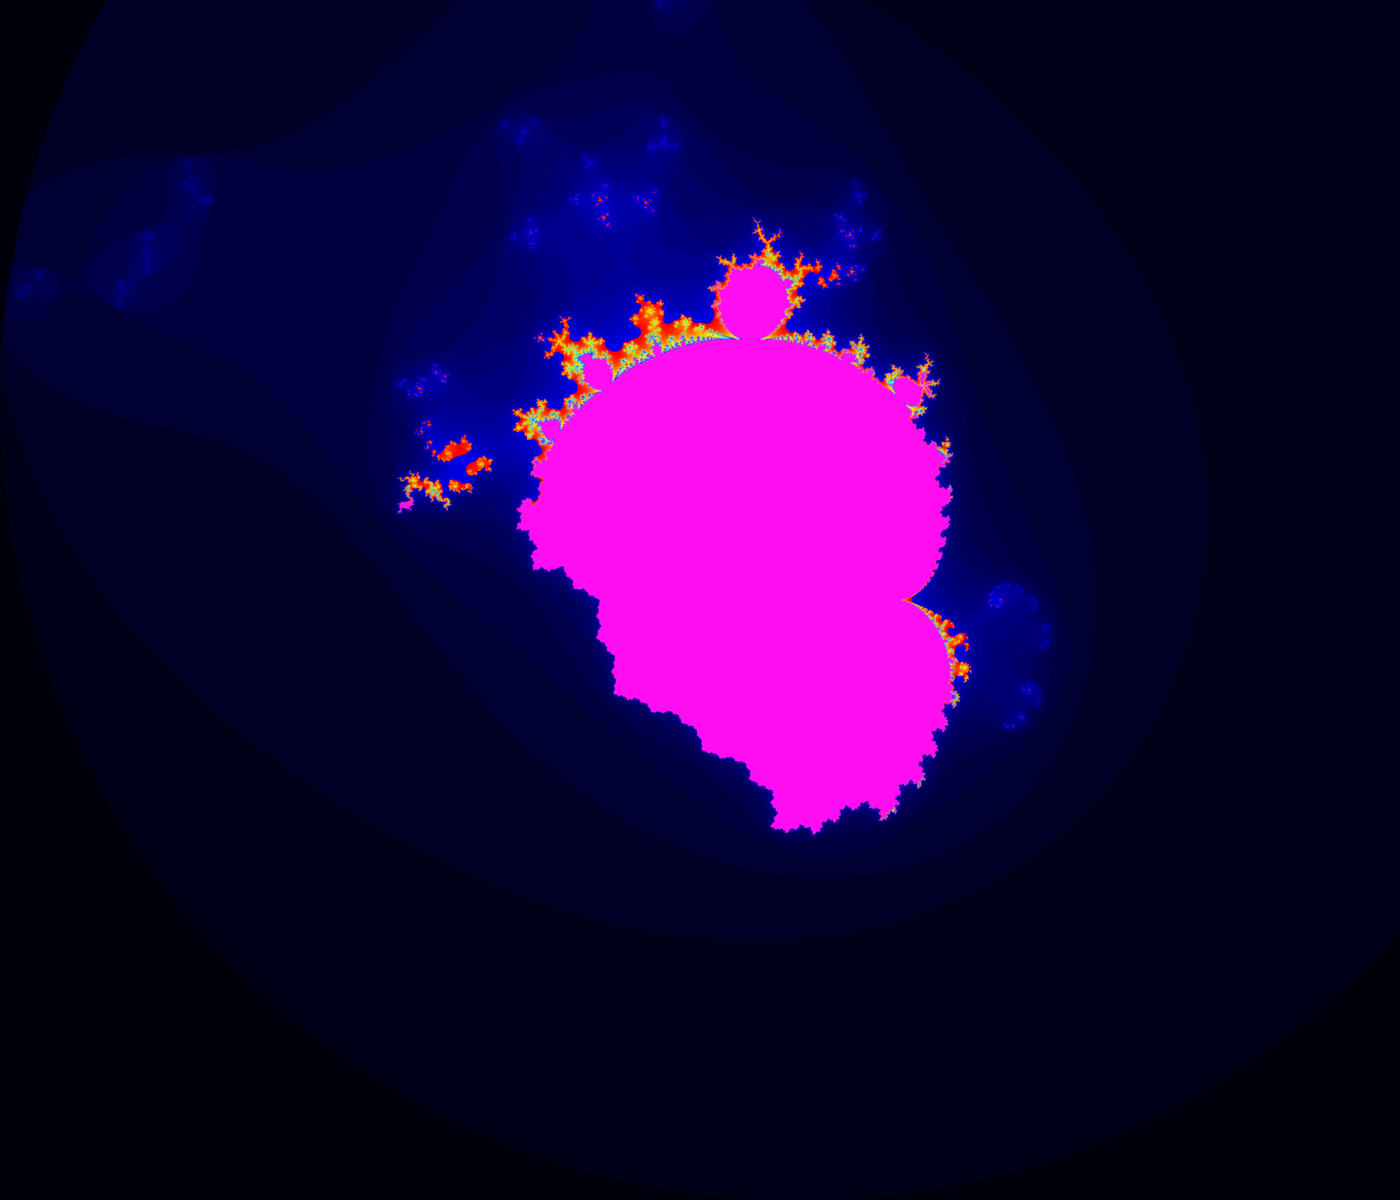
\includegraphics[width=0.3\textwidth]{figures/mandelbrot/exponent-2/mandelbrot-125-iterations-z0(0.500000,0.500000).png}
    }
    \\
    \subfloat[$z_0 = (-0.40, 0.60)$]{
        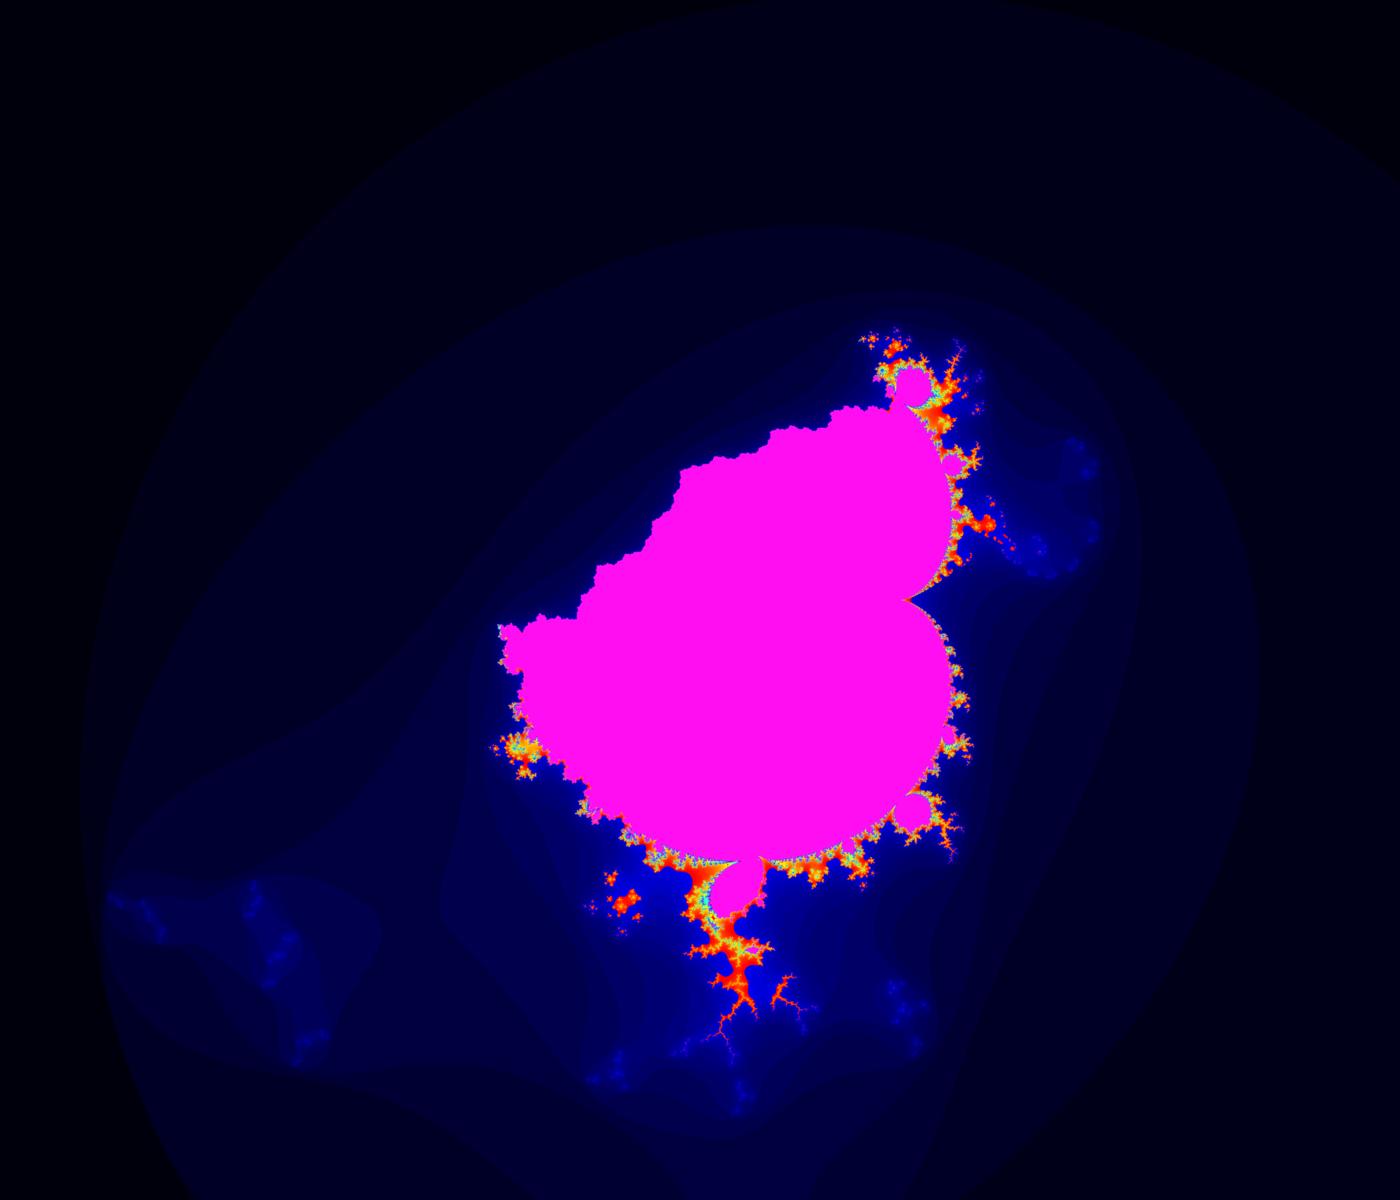
\includegraphics[width=0.3\textwidth]{figures/mandelbrot/exponent-2/mandelbrot-125-iterations-z0(-0.400000,0.600000).png}
    }
    \subfloat[$z_0 = (-0.80, 0.20)$]{
        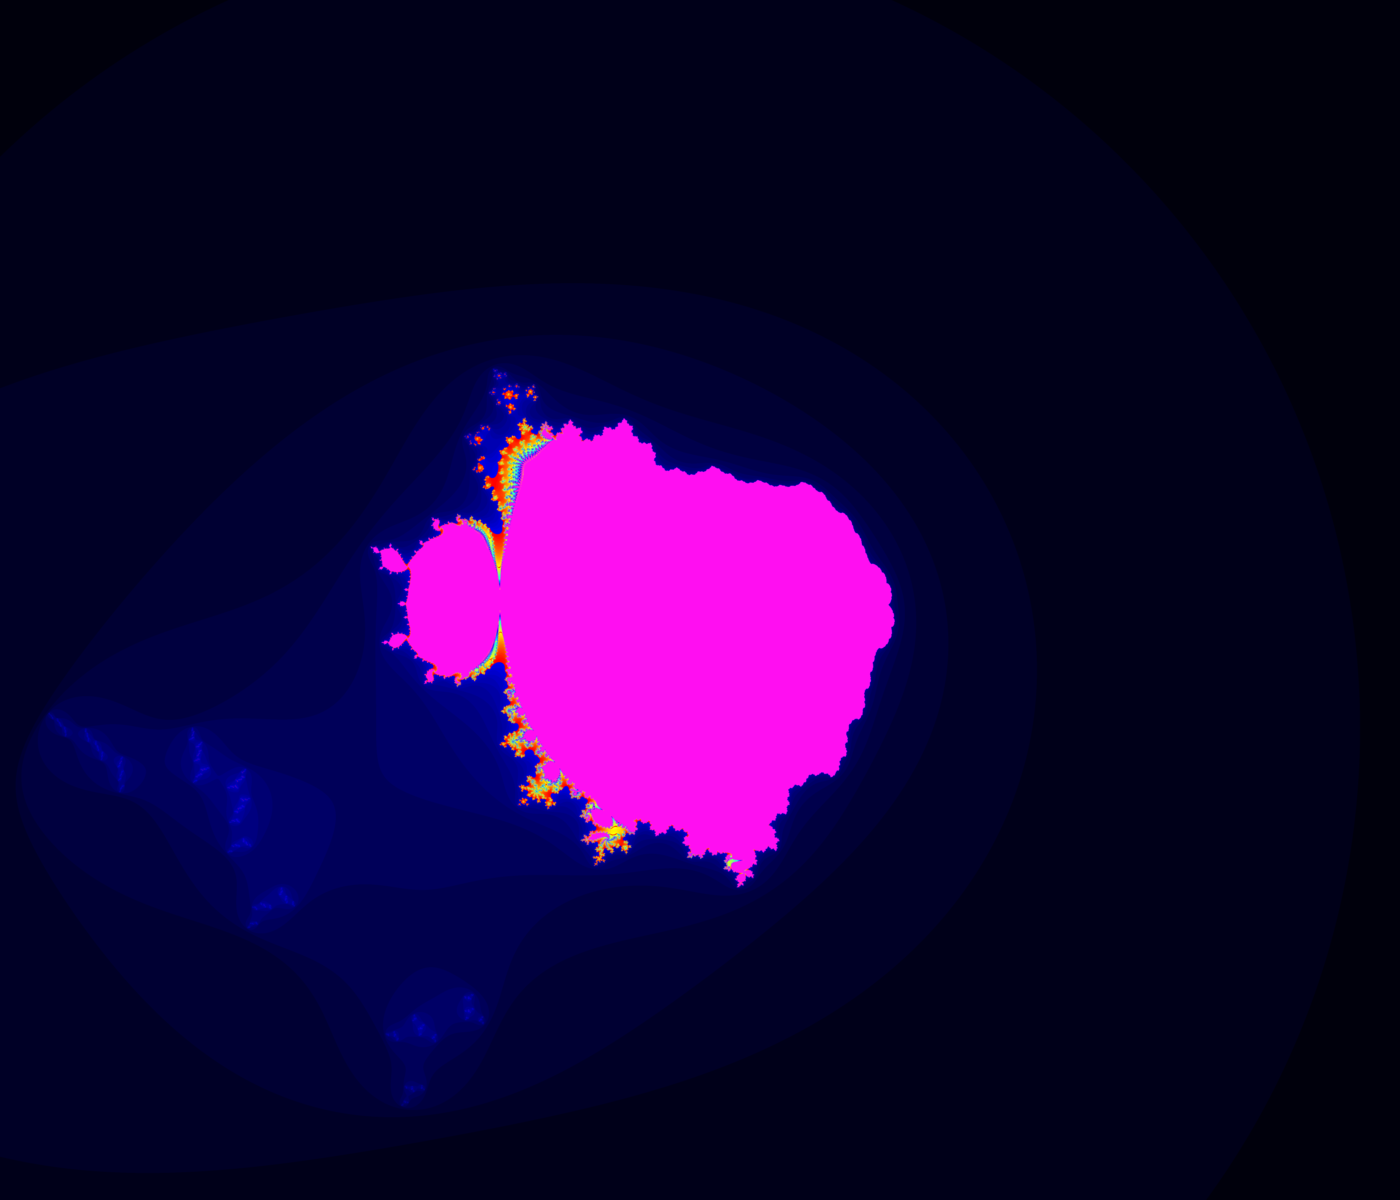
\includegraphics[width=0.3\textwidth]{figures/mandelbrot/exponent-2/mandelbrot-125-iterations-z0(-0.800000,0.200000).png}
    }
    \subfloat[$z_0 = (0.70, 0.70)$]{
        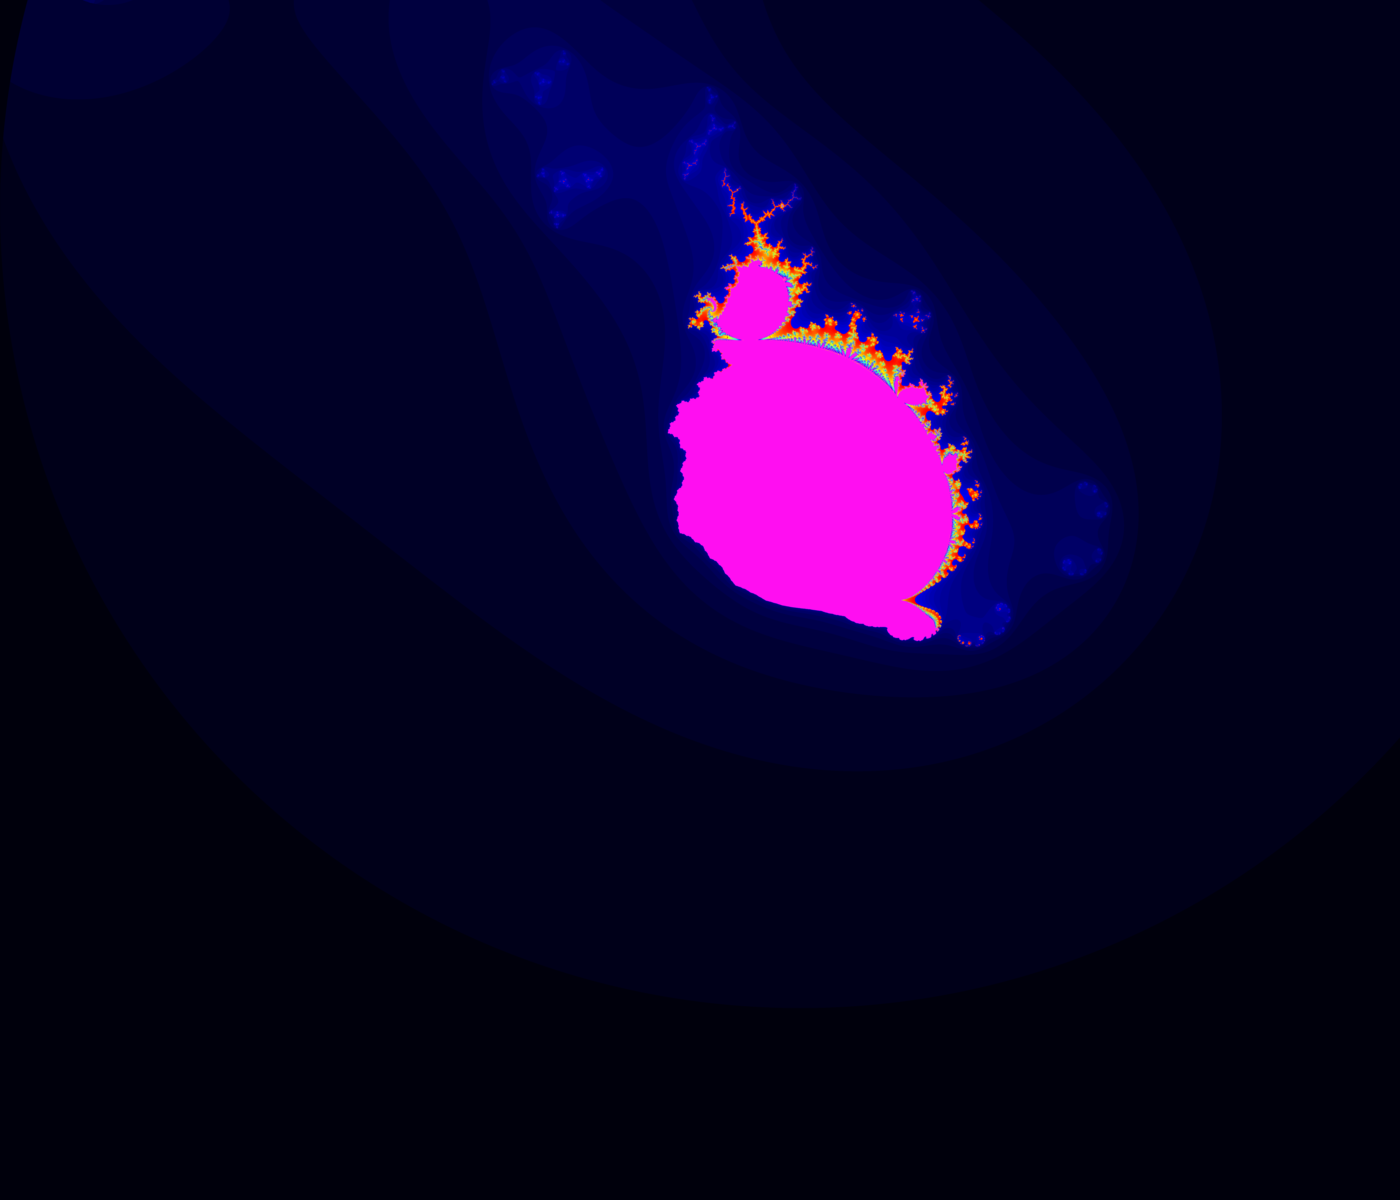
\includegraphics[width=0.3\textwidth]{figures/mandelbrot/exponent-2/mandelbrot-125-iterations-z0(0.700000,0.700000).png}
    }
    \caption{Conjuntos de Mandelbrot para diferentes valores de $z_0$ e iterações. Cada subfigura apresenta o conjunto gerado para o respectivo valor de $z_0$.}
\end{figure}  

    \begin{table}[H]
        \centering
        \caption{Índice das imagens, valores de $z_0$ e módulo de $z_0$.}
        \begin{tabular}{|c|c|c|}
            \hline
            Índice & $z_0$ & $|z_0|$ \\ \hline
            (a) & $(0.30, 0.10)$ & $\sqrt{0.30^2 + 0.10^2} \approx 0.316$ \\ \hline
            (b) & $(0.30, 0.50)$ & $\sqrt{0.30^2 + 0.50^2} \approx 0.583$ \\ \hline
            (d) & $(0.50, 0.50)$ & $\sqrt{0.50^2 + 0.50^2} \approx 0.707$ \\ \hline
            (c) & $(-0.40, 0.60)$ & $\sqrt{(-0.40)^2 + 0.60^2} \approx 0.721$ \\ \hline
            (e) & $(-0.80, 0.20)$ & $\sqrt{(-0.80)^2 + 0.20^2} \approx 0.824$ \\ \hline
            (f) & $(0.70, 0.70)$ & $\sqrt{0.70^2 + 0.70^2} \approx 0.990$ \\ \hline
        \end{tabular}
    \end{table}

    Uma análise interessante é que, à medida que o valor de \(|z_0|\) aumenta, o conjunto de Mandelbrot aparenta diminuir em tamanho (redução da área de cor rosa na figura). Isso possivelmente ocorre devido à maior probabilidade de os valores iterados escaparem para o infinito, reduzindo a região de convergência.   
    
    
\item[(c)] Pode-se também alterar a forma de observar a dinâmica: ao invés de fixar a condição inicial $z_0$, escolha um valor fixo para $c$ e estude as órbitas variando os valores de $z_0$, escolhendo aqueles para os quais a função $f_c^n(z_0)$ não diverge quando $n \to \infty$. Plote alguns exemplos desse novo fractal. Os fractais gerados nessa questão e na anterior são exemplos dos conhecidos conjuntos de Julia.

\begin{figure}[H]
        \centering
        \subfloat[$c = (0.355, 0.337)$]{
                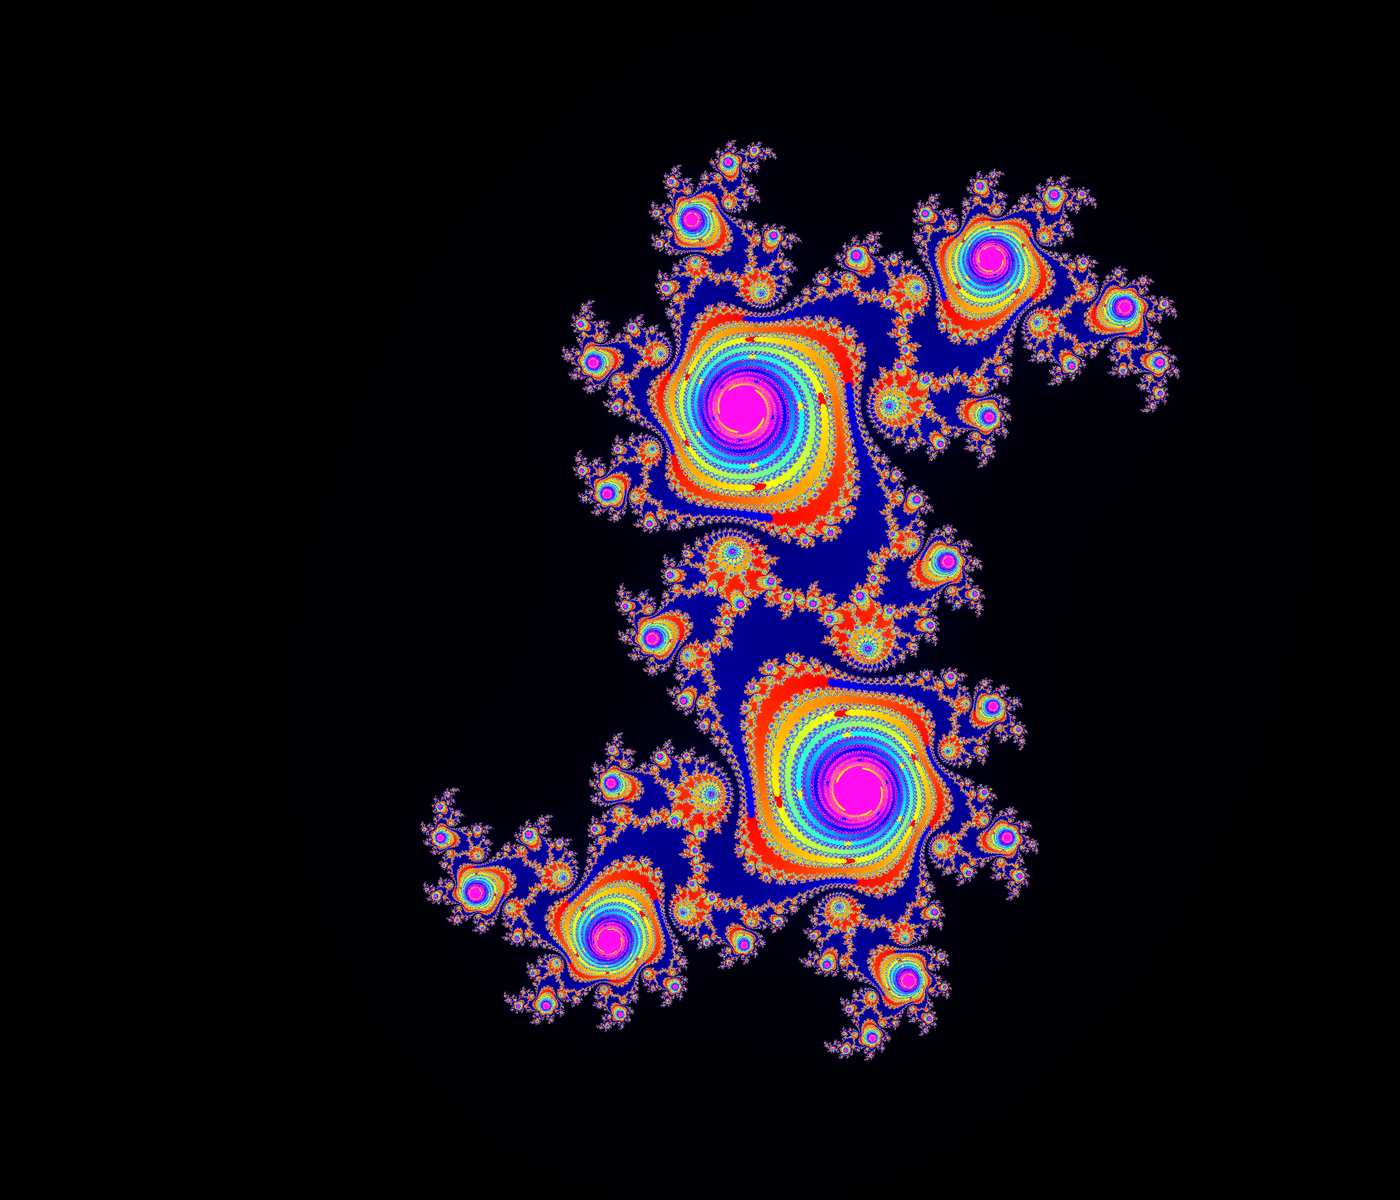
\includegraphics[width=0.3\textwidth]{figures/julia/julia-1000-iterations-c(0.355000,0.337000).png}
        }
        \subfloat[$c = (0.370, -0.100)$]{
                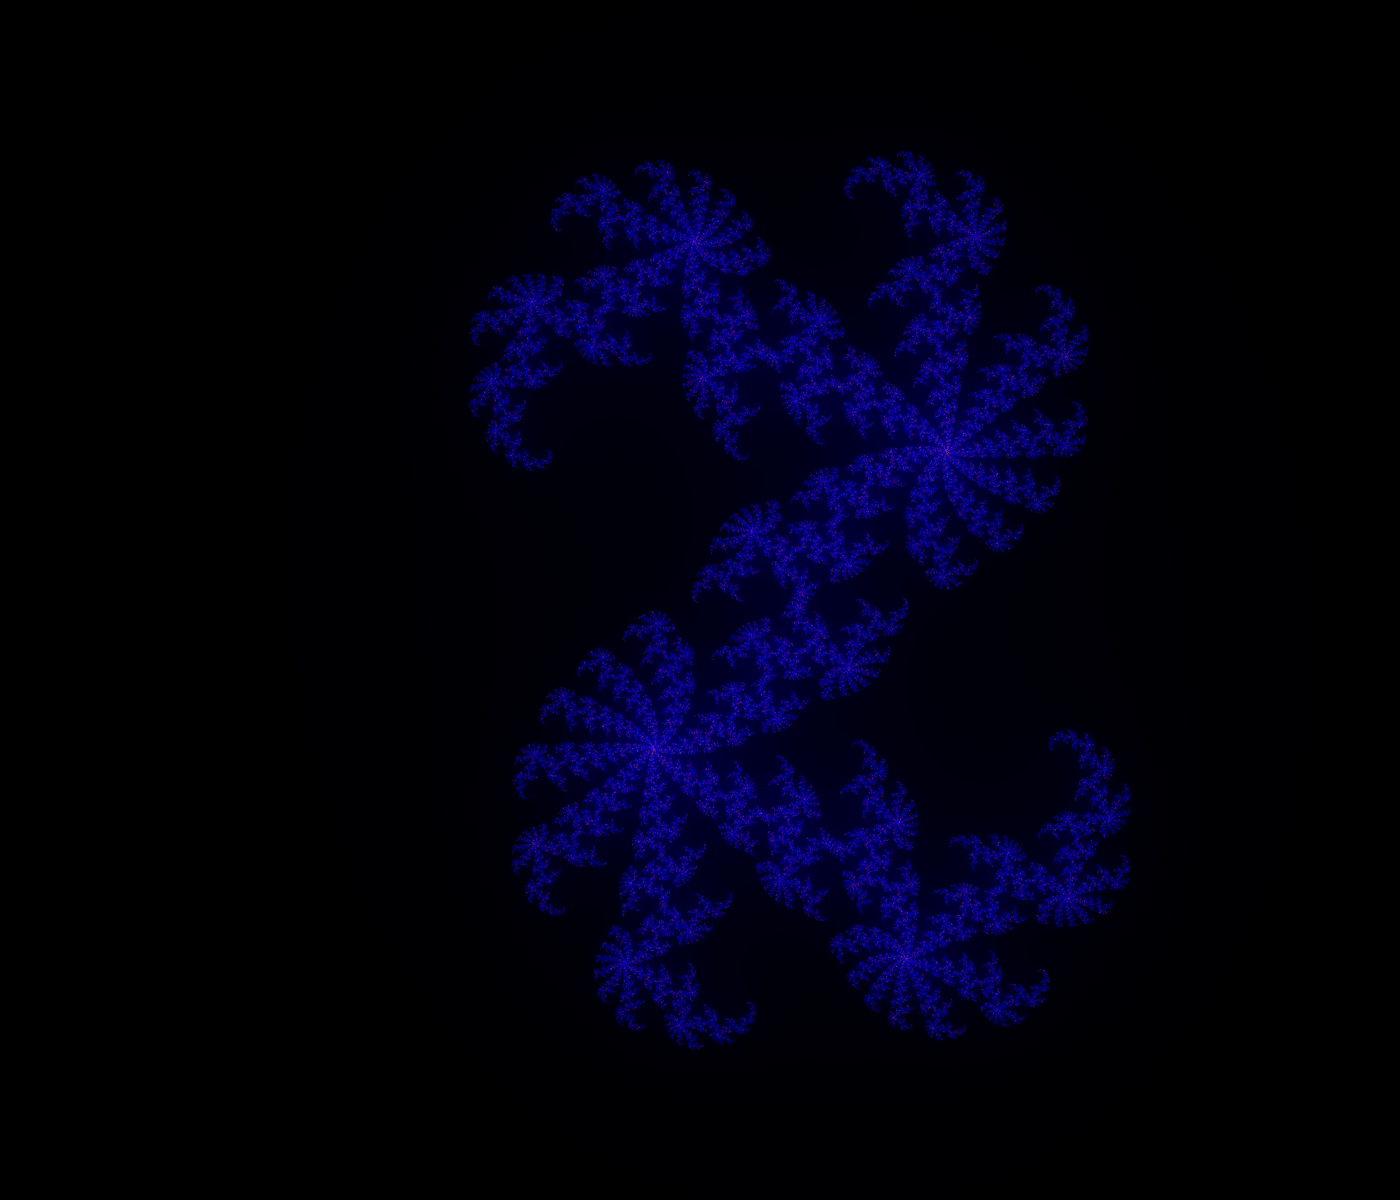
\includegraphics[width=0.3\textwidth]{figures/julia/julia-1000-iterations-c(0.370000,-0.100000).png}
        }
        \subfloat[$c = (-0.800, 0.156)$]{
                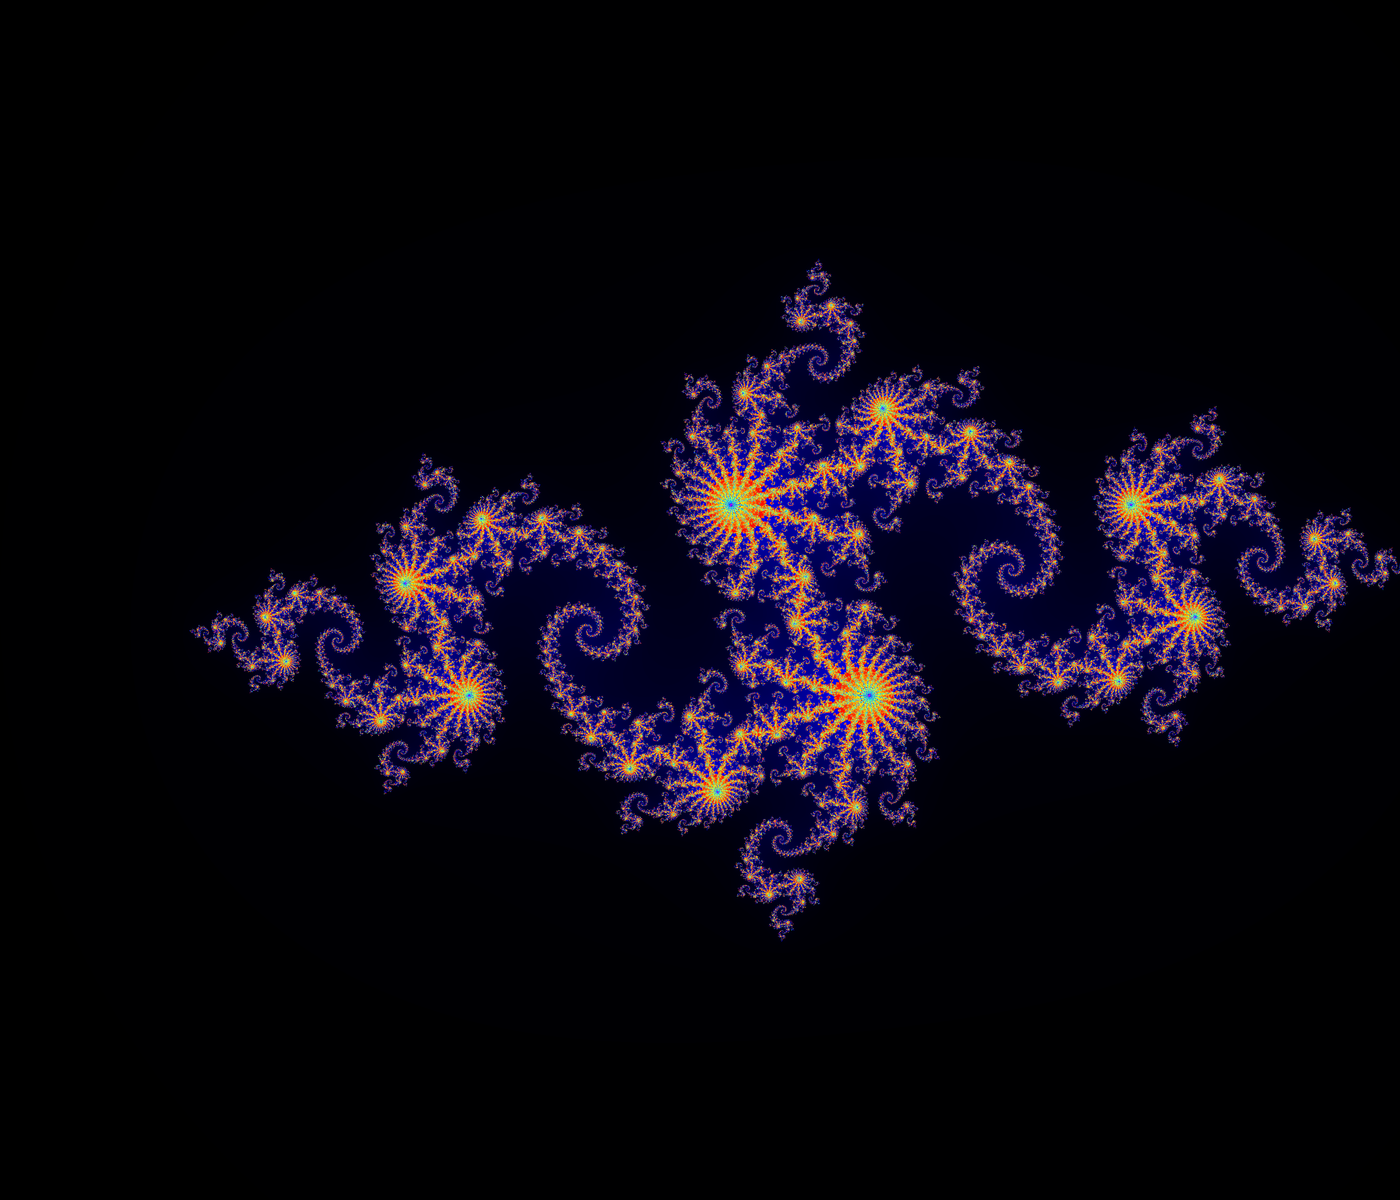
\includegraphics[width=0.3\textwidth]{figures/julia/julia-1000-iterations-c(-0.800000,0.156000).png}
        }
        \caption{Conjuntos de Julia para diferentes valores de $c$ utilizando o expoente $d = 2$. Cada subfigura apresenta o conjunto gerado para o respectivo valor de $c$.}
\end{figure}

\begin{figure}[H]
        \centering
        \subfloat[$c = (0.450, 0.1428)$, expoente $d = -1$]{
                
\includegraphics[width=0.3\textwidth]{figures/julia/julia-125-iterations-c(0.450000,0.142800)--1.png}
        }
        \subfloat[$c = (0.500, 0.500)$, expoente $d = 3$]{       
                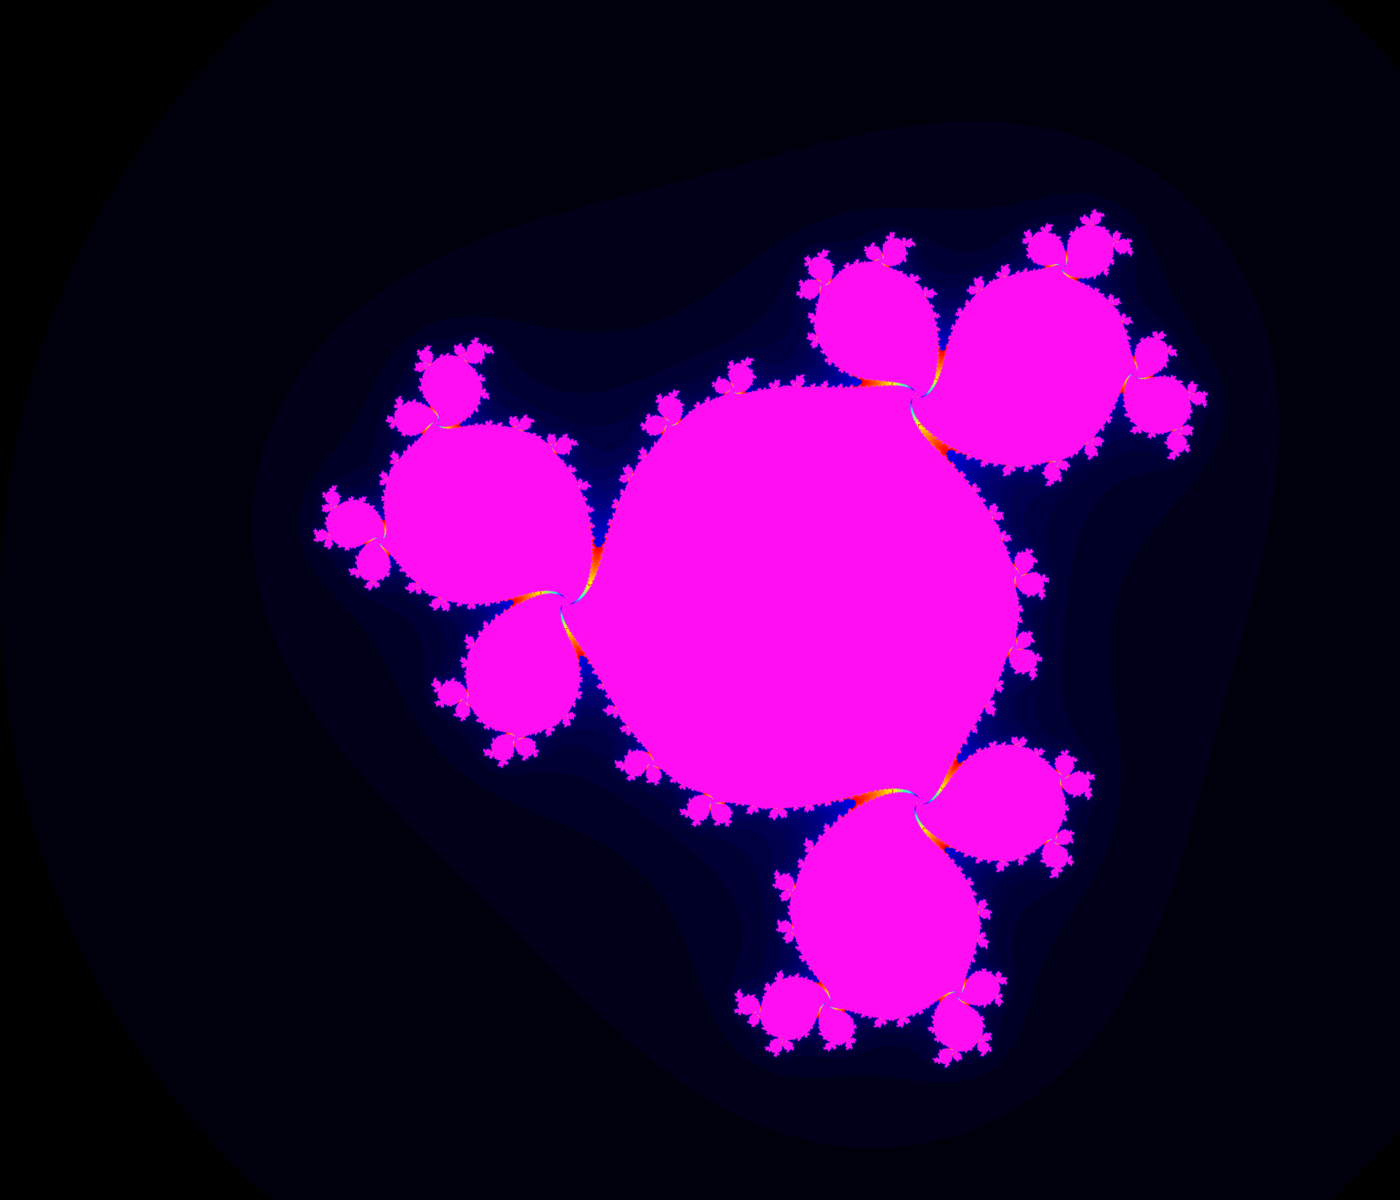
\includegraphics[width=0.3\textwidth]{figures/julia/julia-125-iterations-c(0.500000,0.500000)-e-3.png}
        }
        \subfloat[$c = (0.500, 0.500)$, expoente $d = 7$]{
                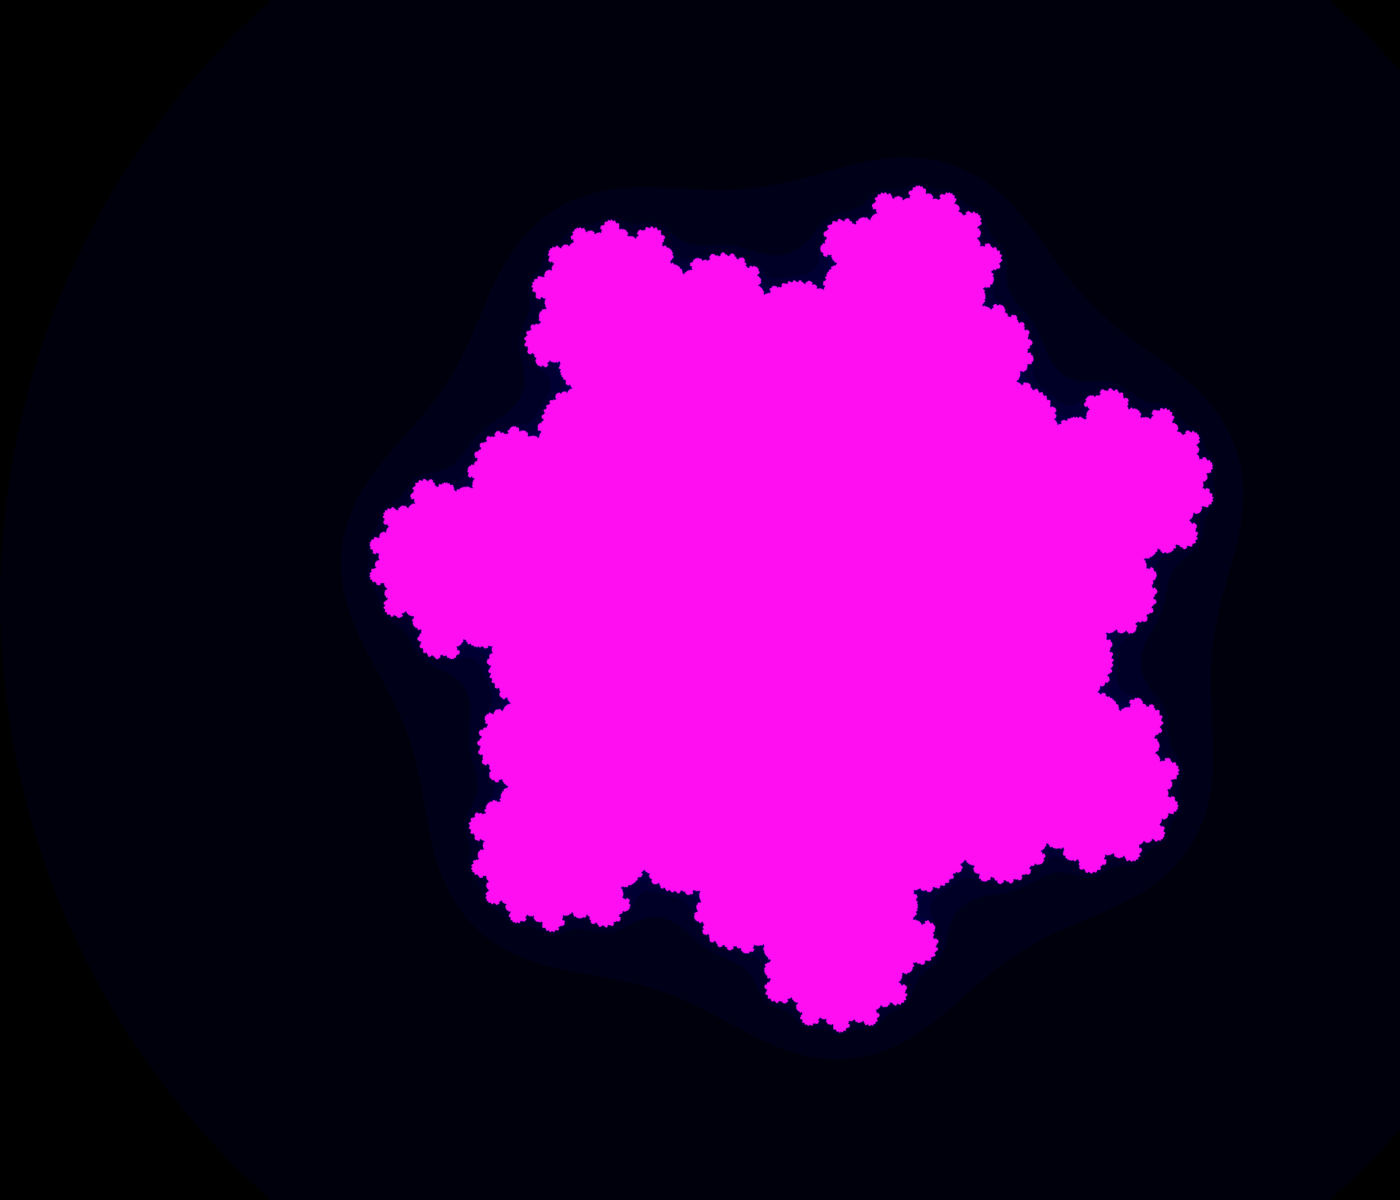
\includegraphics[width=0.3\textwidth]{figures/julia/julia-125-iterations-c(0.500000,0.500000)-e-7.png}
        }
        \caption{Conjuntos de Julia para diferentes valores de $c$ e expoentes.}
\end{figure}


Para todos os exemplos apresentados, foram utilizadas 125 iterações, e os valores iniciais estão indicados nas legendas das figuras correspondentes. Essa uniformidade nos parâmetros permite uma análise comparativa mais clara entre as diferentes variações dos conjuntos de Mandelbrot, Julia e Multibrot, destacando como as alterações nos valores de $z_0$, $c$ e $d$ influenciam as formas e os padrões gerados.

\item[(d)] Uma terceira forma de alterar $M$ é mudando o grau do polinômio $f_c$, substituindo $d$ na função $f_c(z) = z^d + c$ por outros números positivos. Veja o que acontece com a figura ao usar diferentes valores. Esses conjuntos são conhecidos como \emph{Multibrot}. Experimente também valores negativos de $d$.


\begin{figure}[H]
        \centering
        \subfloat[Exponente $d = -1$]{
                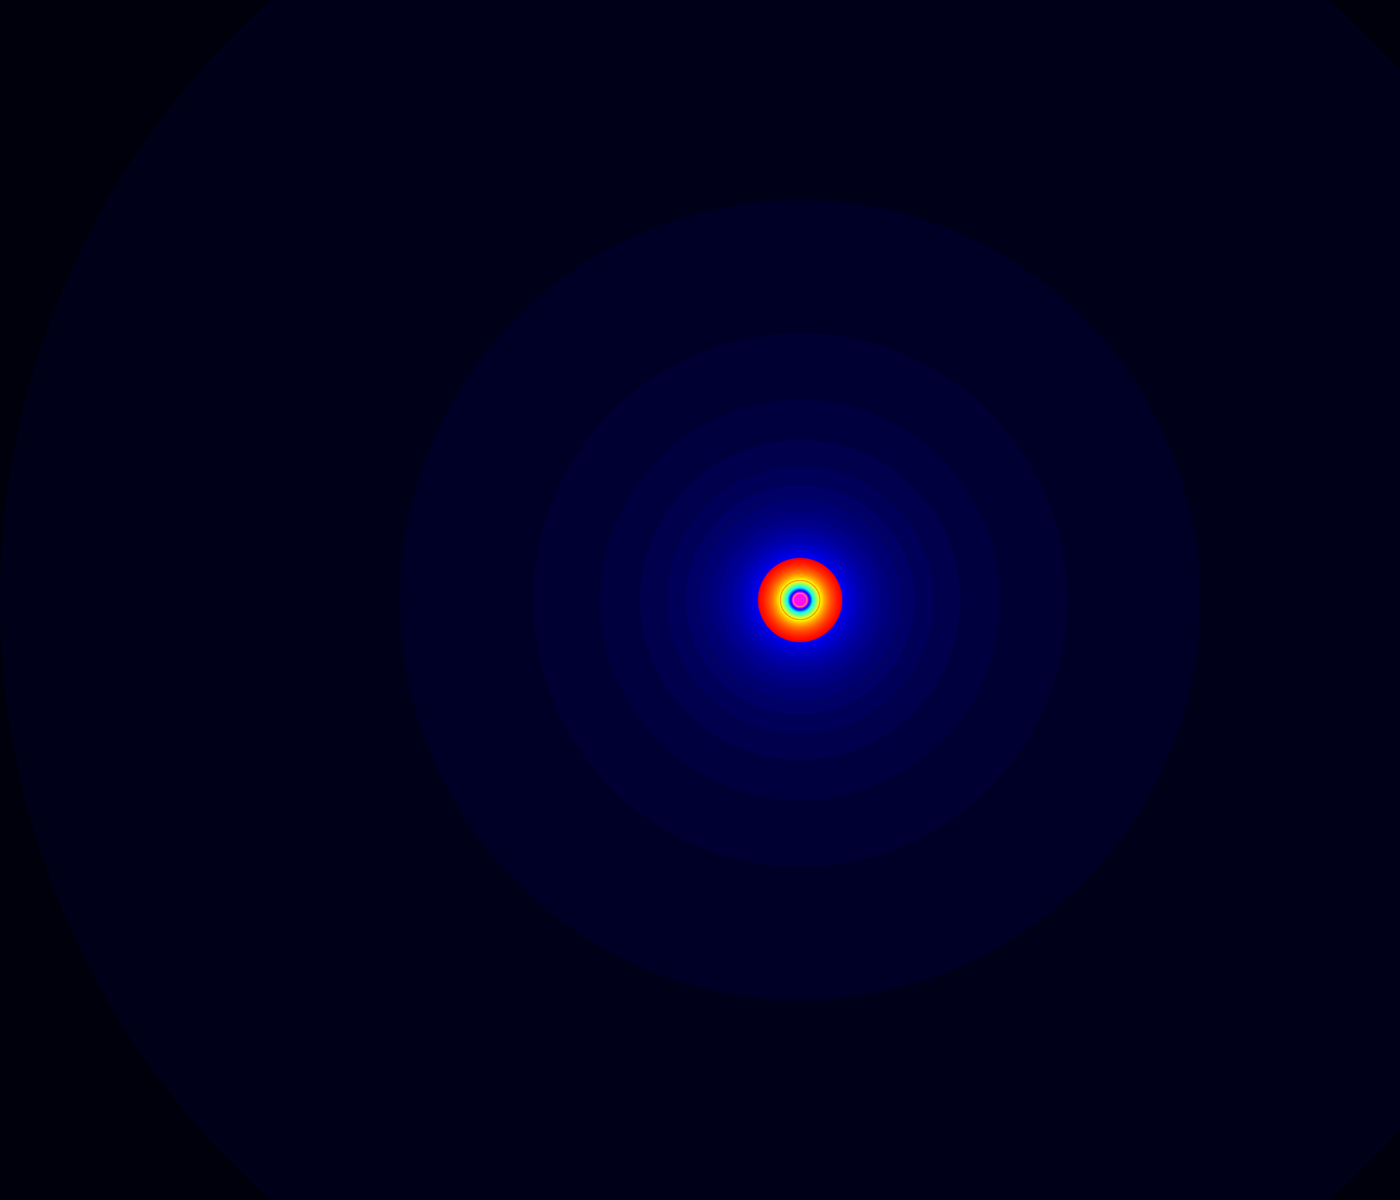
\includegraphics[width=0.3\textwidth]{figures/mandelbrot/exponent-d/mandelbrot-125-iterations-exponent--1.png}
        }
        \subfloat[Exponente $d = 2$]{
                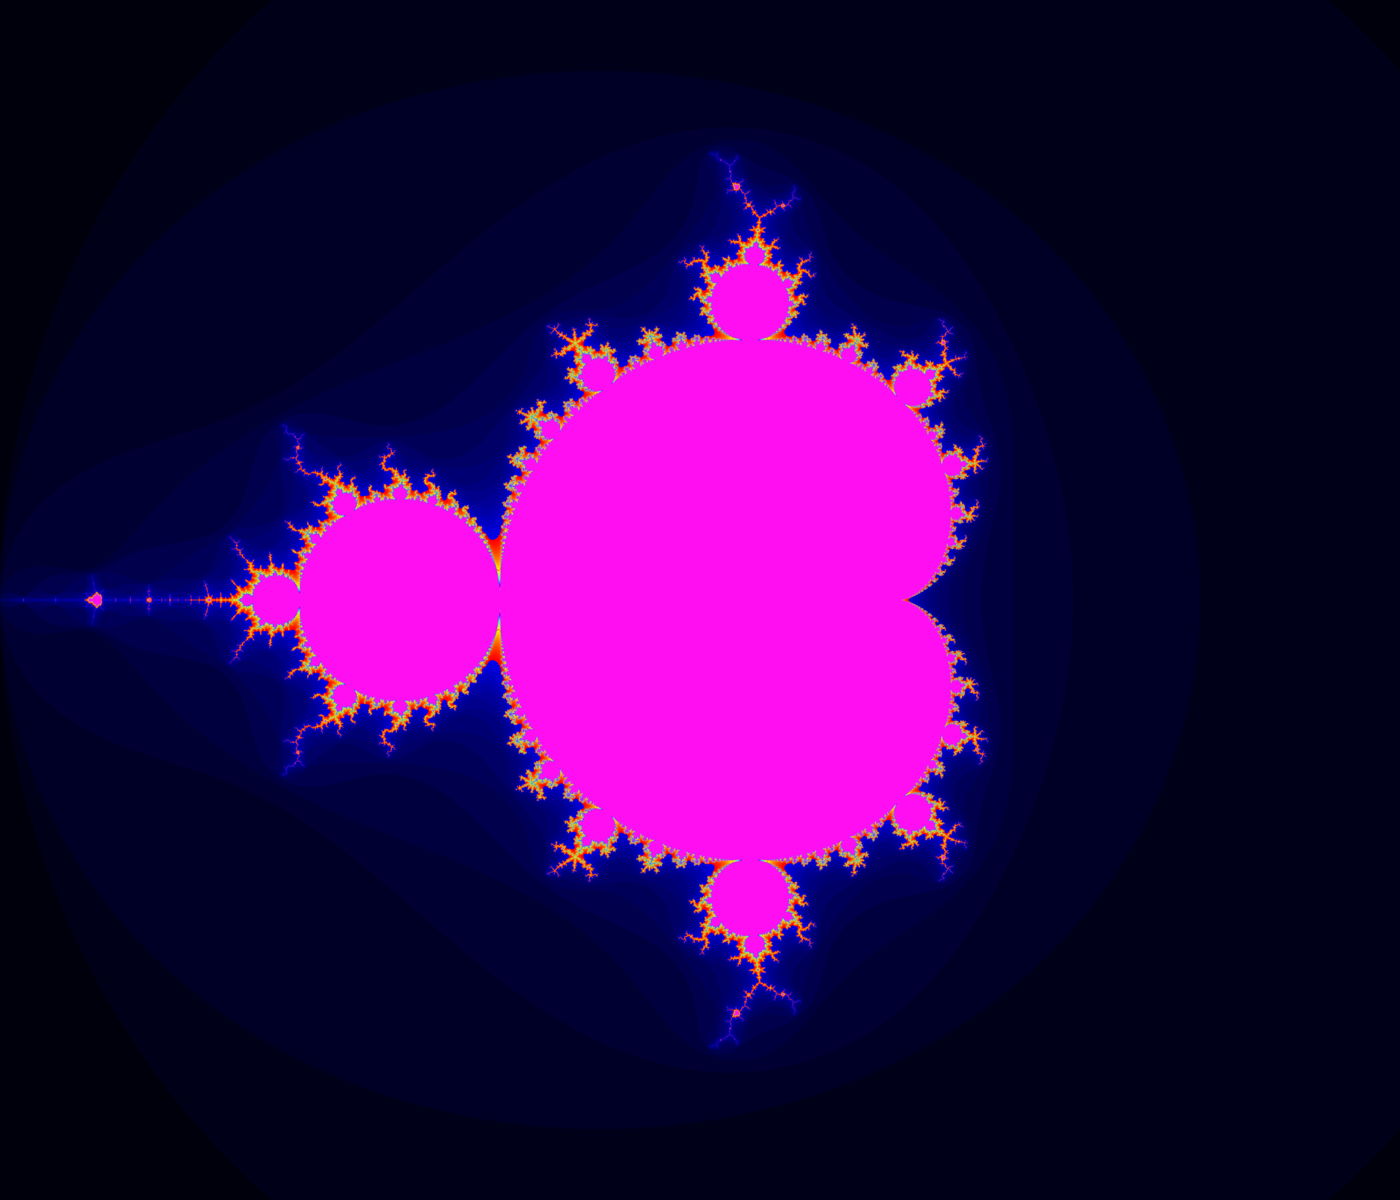
\includegraphics[width=0.3\textwidth]{figures/mandelbrot/exponent-d/mandelbrot-125-iterations-exponent-2.png}
        }
        \subfloat[Exponente $d = 4$]{
                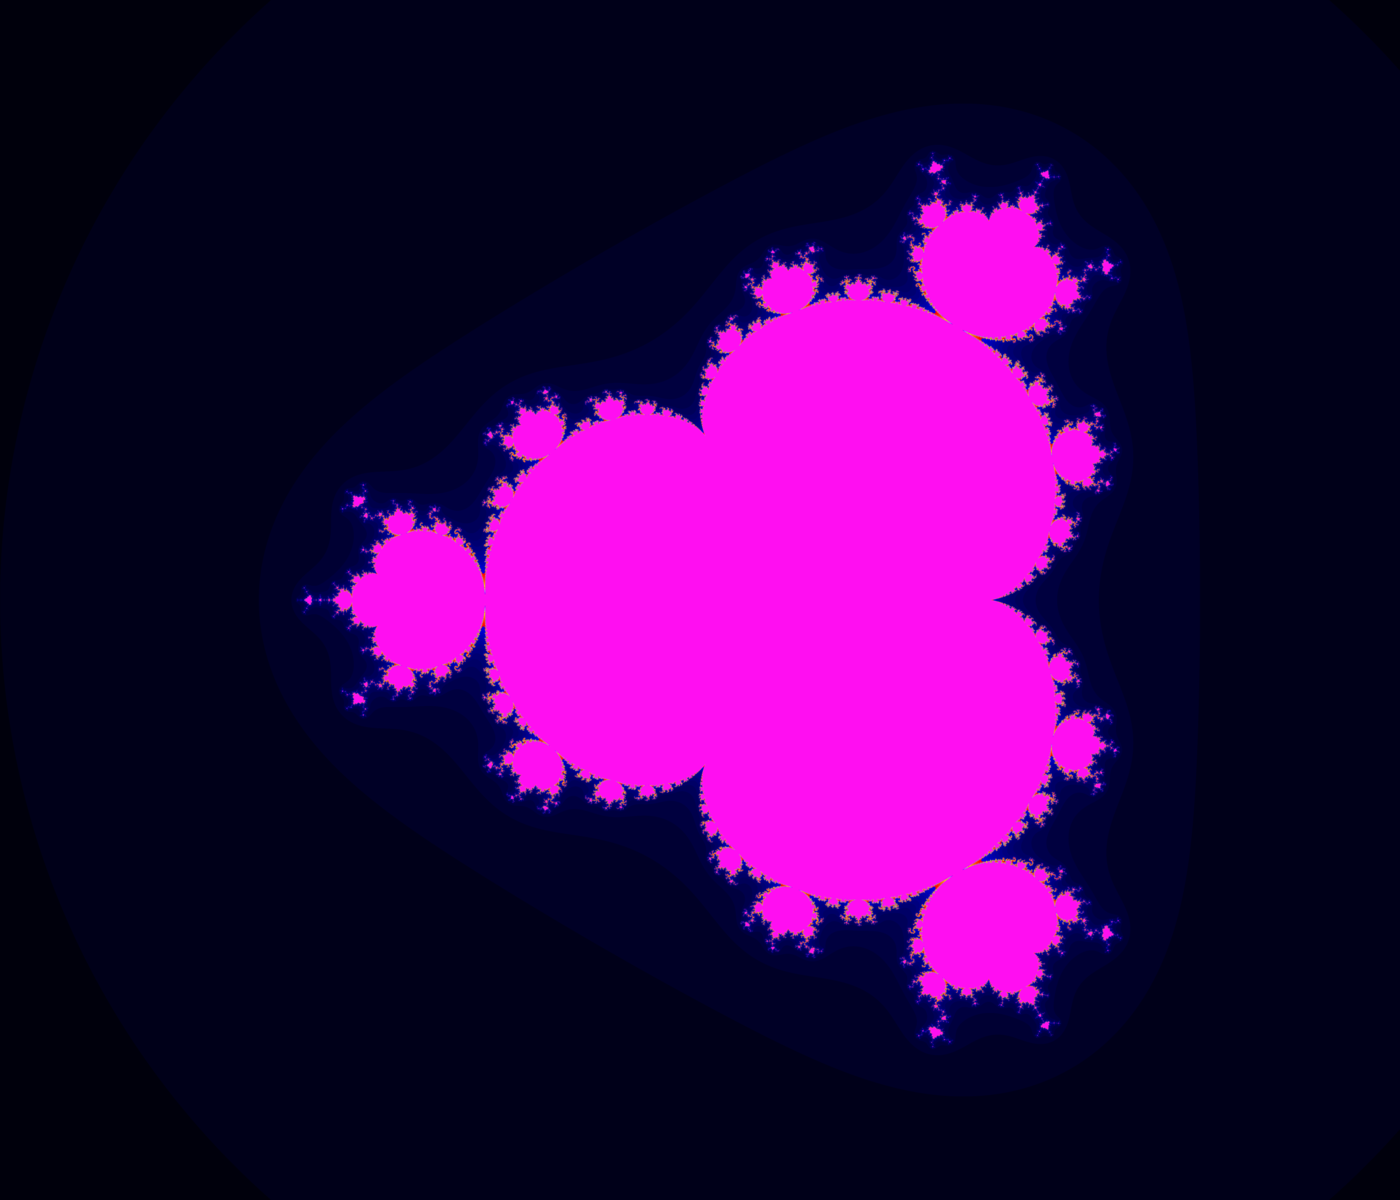
\includegraphics[width=0.3\textwidth]{figures/mandelbrot/exponent-d/mandelbrot-125-iterations-exponent-4.png}
        }
        \\
        \subfloat[Exponente $d = 5$]{
                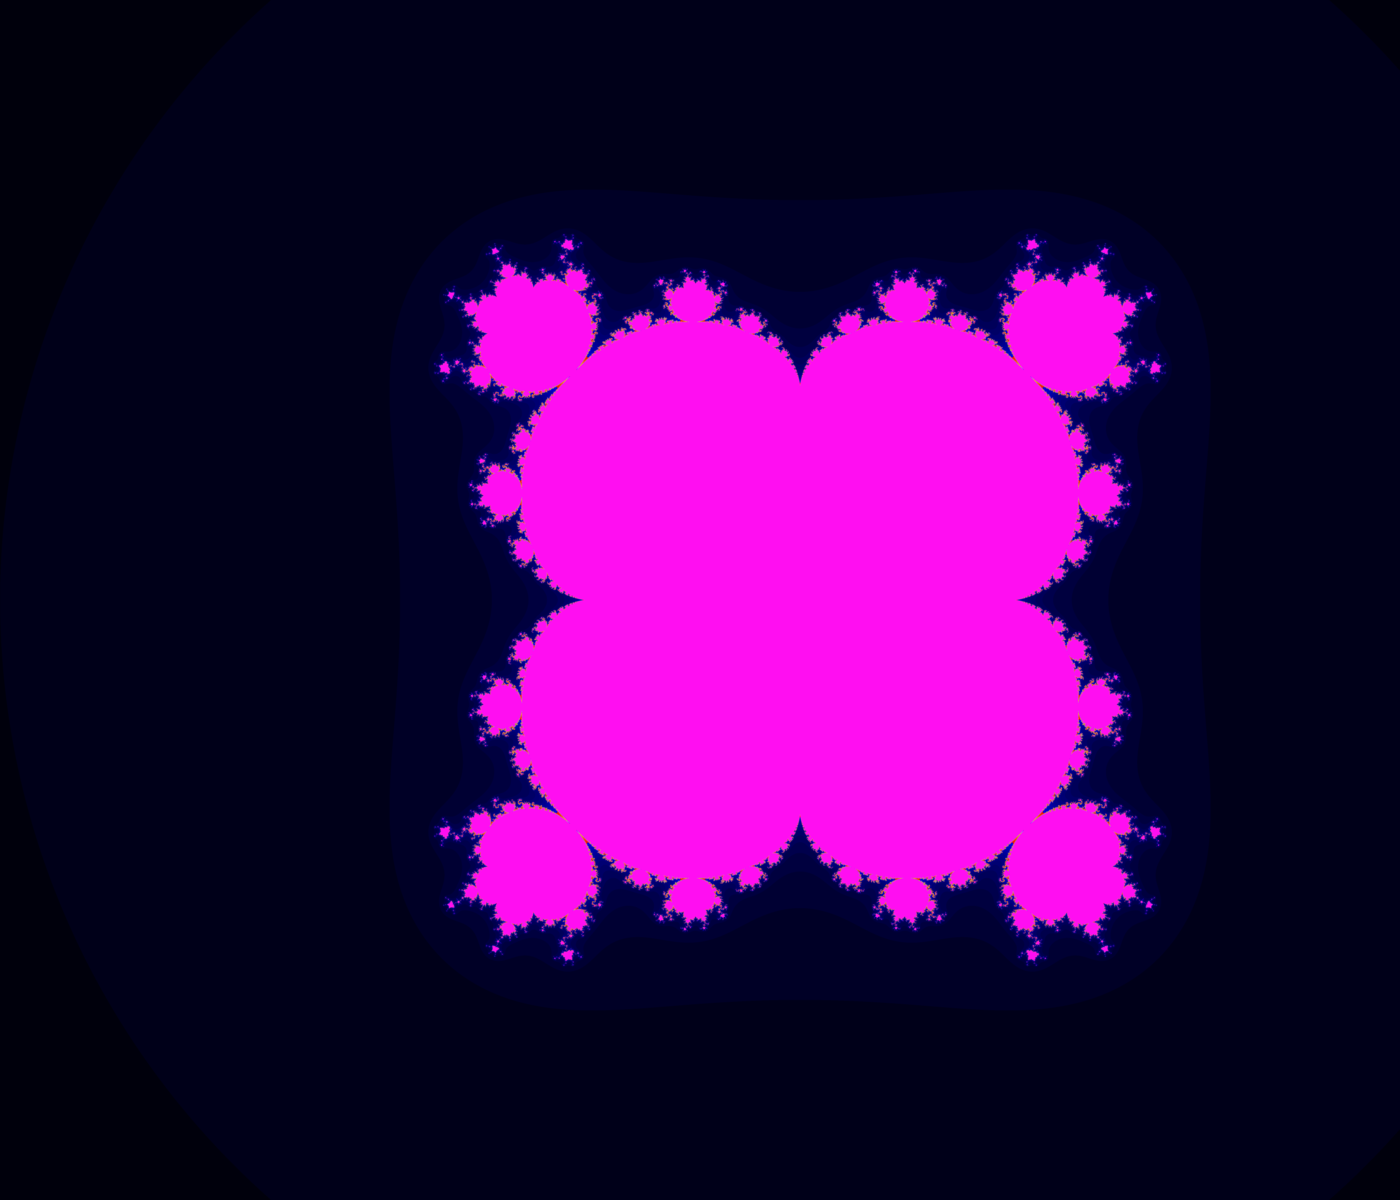
\includegraphics[width=0.3\textwidth]{figures/mandelbrot/exponent-d/mandelbrot-125-iterations-exponent-5.png}
        }
        \subfloat[Exponente $d = 6$]{
                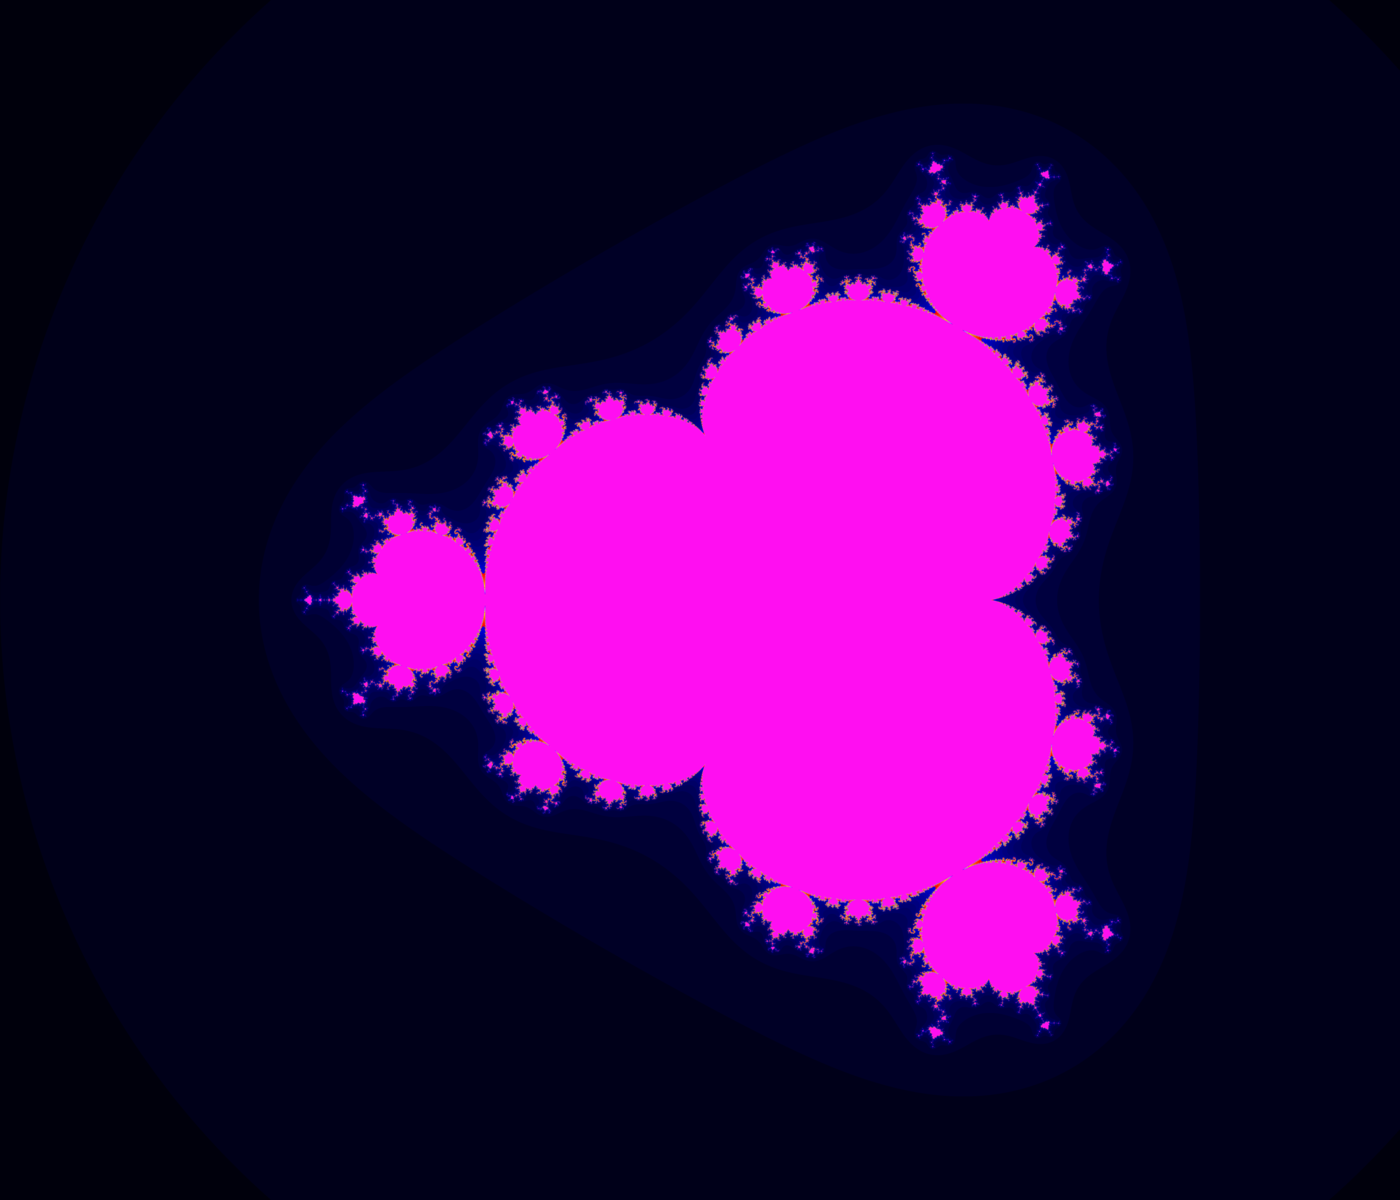
\includegraphics[width=0.3\textwidth]{figures/mandelbrot/exponent-d/mandelbrot-125-iterations-exponent-6.png}
        }
        \subfloat[Exponente $d = 13$]{
                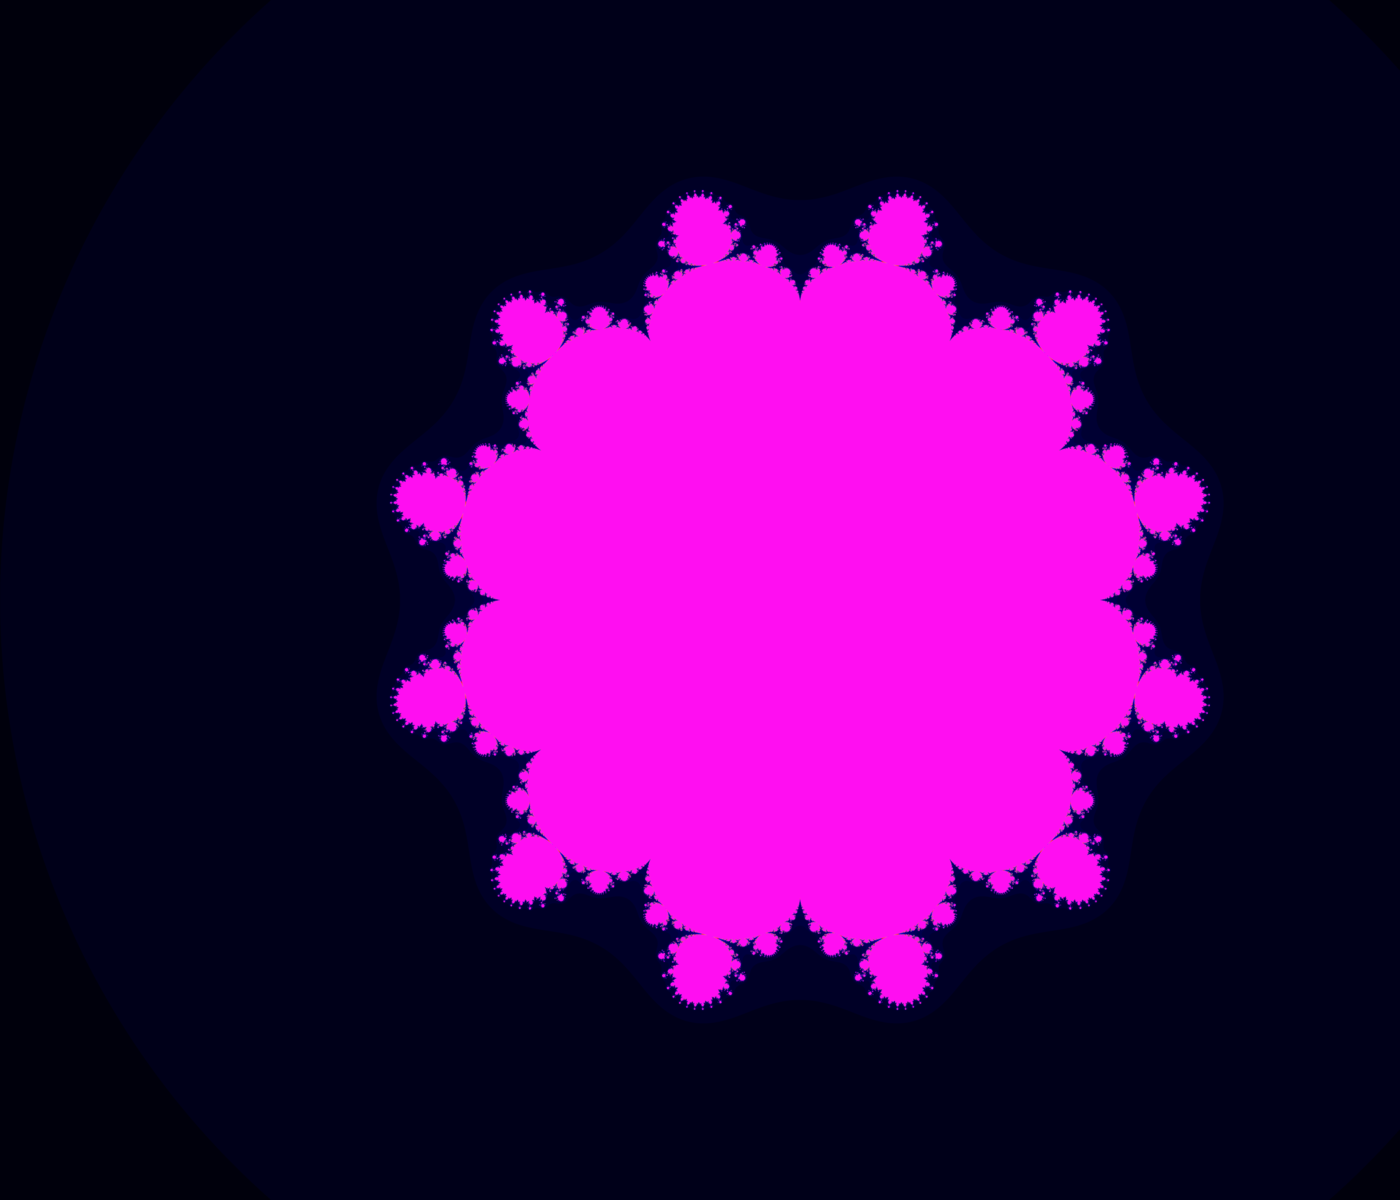
\includegraphics[width=0.3\textwidth]{figures/mandelbrot/exponent-d/mandelbrot-125-iterations-exponent-13.png}
        }
        \\
        \subfloat[Exponente $d = 37$]{
                
\includegraphics[width=0.3\textwidth]{figures/mandelbrot/exponent-d/mandelbrot-125-iterations-exponent-37.png}
        }
        \subfloat[Exponente $d = 50$]{
                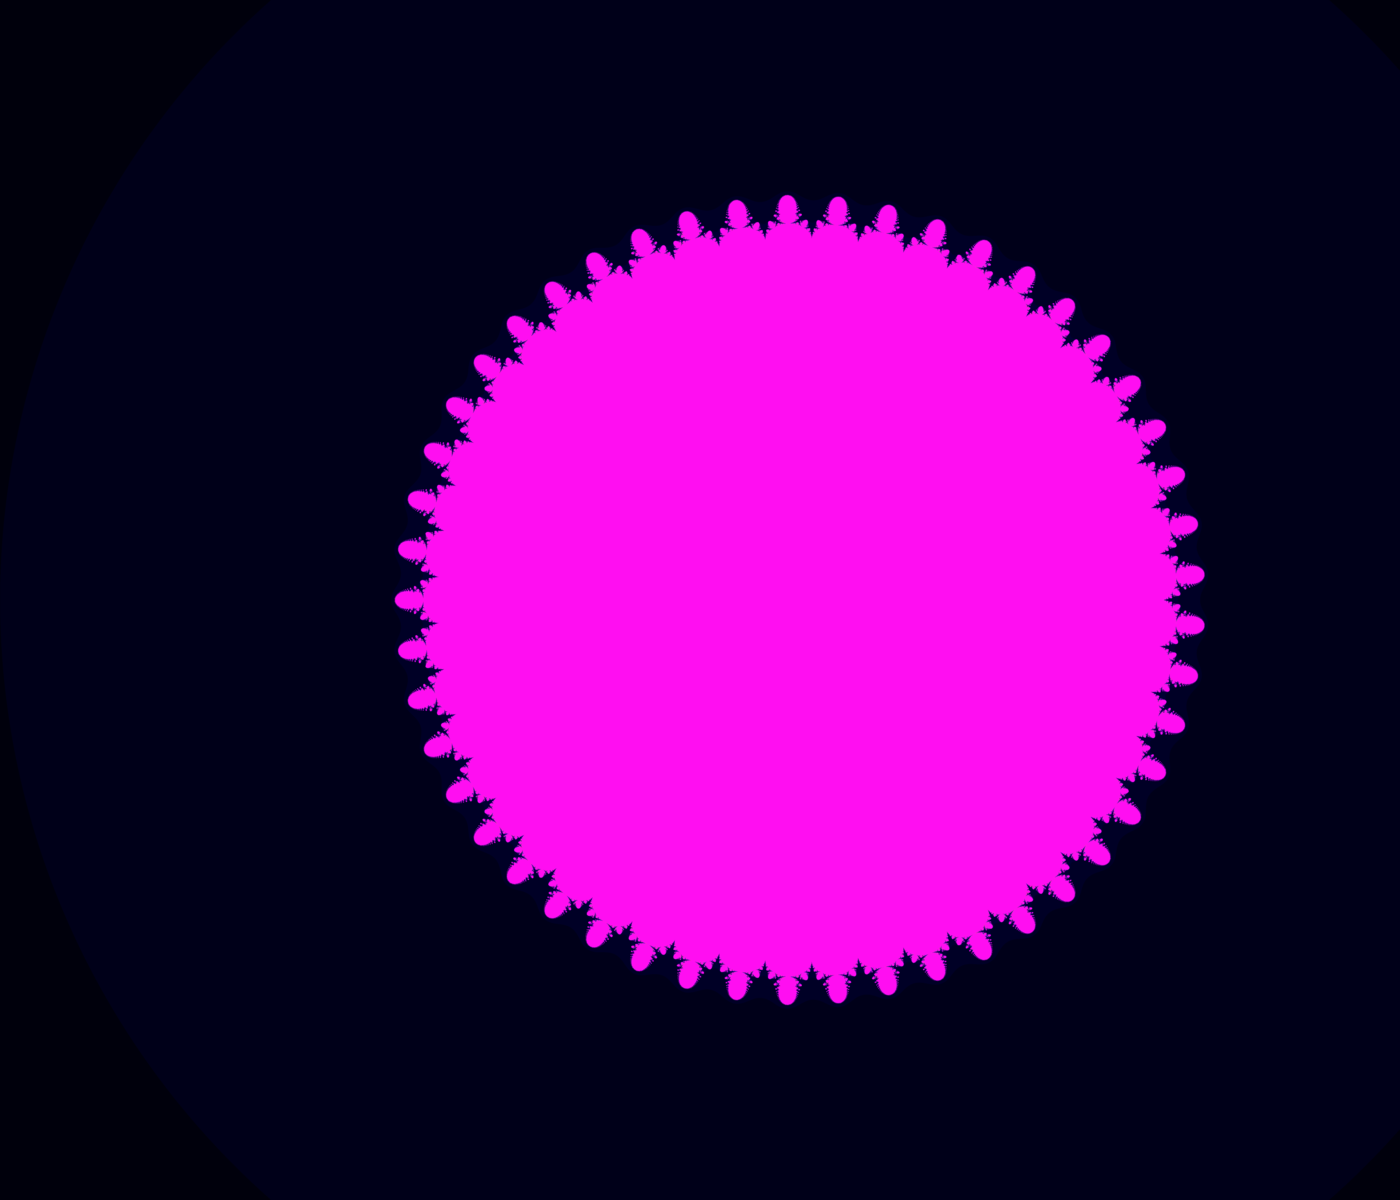
\includegraphics[width=0.3\textwidth]{figures/mandelbrot/exponent-d/mandelbrot-125-iterations-exponent-50.png}
        }
        \subfloat[Exponente $d = 100$]{
                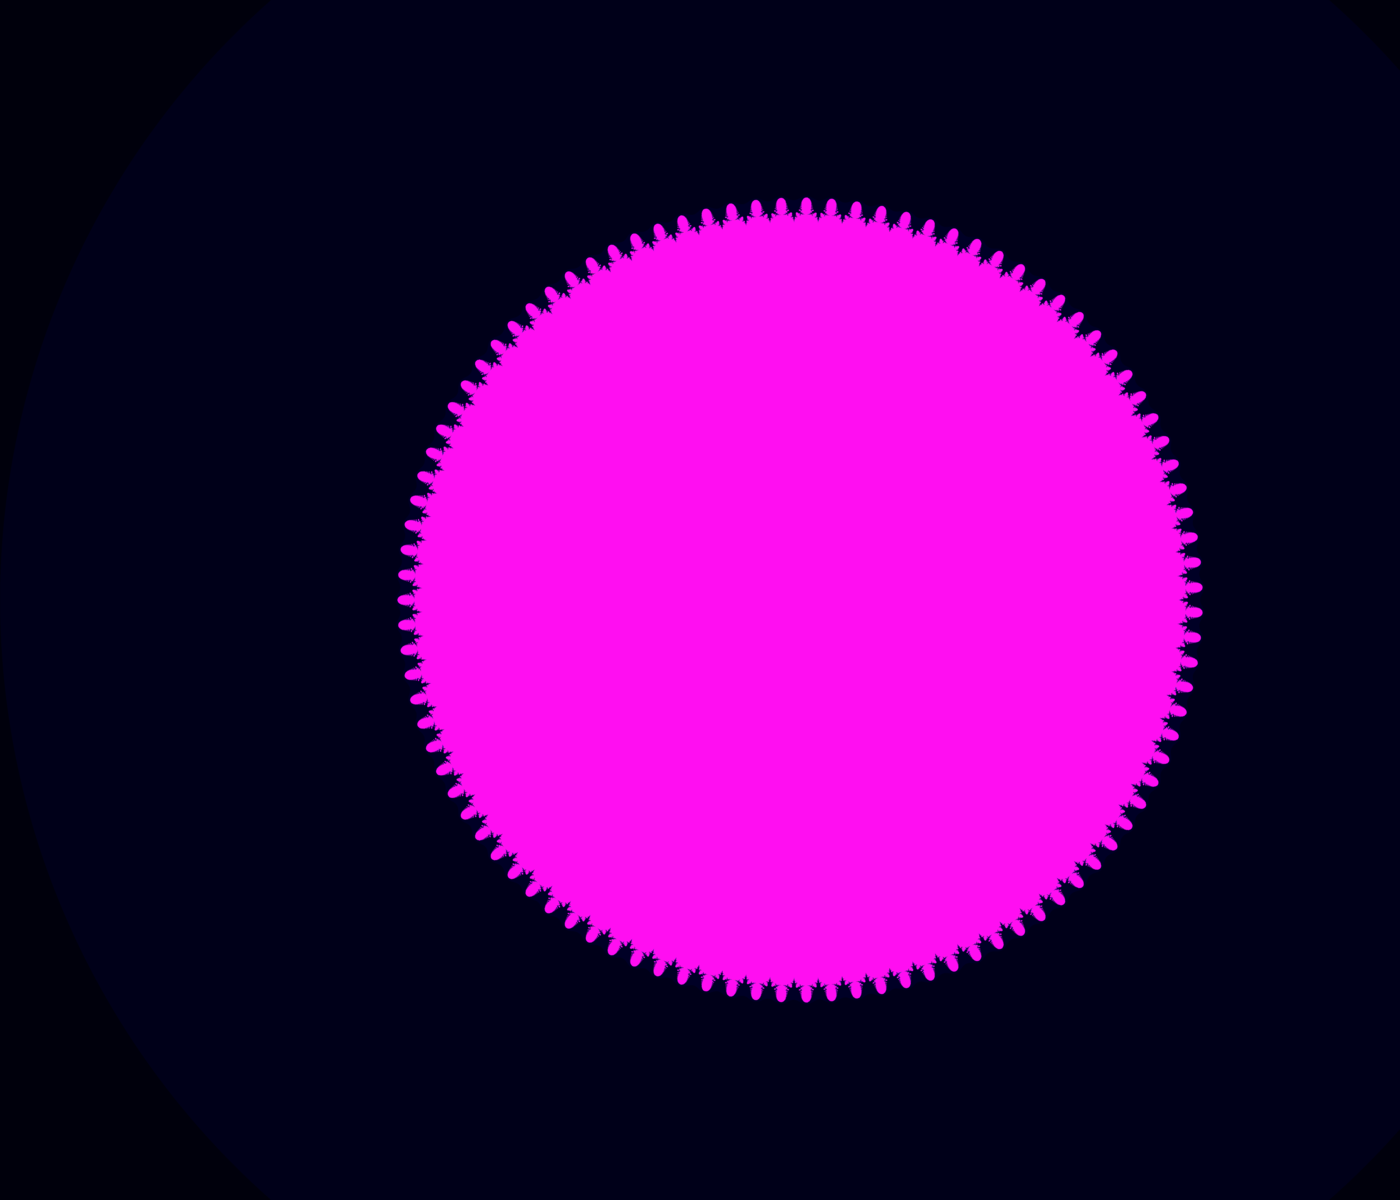
\includegraphics[width=0.3\textwidth]{figures/mandelbrot/exponent-d/mandelbrot-125-iterations-exponent-100.png}
        }
        \caption{Conjuntos de Mandelbrot para diferentes valores do exponente $d$. Cada subfigura apresenta o conjunto gerado para o respectivo valor de $d$.}
\end{figure} 

        Uma análise interessante sobre os conjuntos de Mandelbrot gerados para diferentes valores do expoente $d$ é a simetria presente nas figuras. Para valores positivos de $d$, observa-se que os conjuntos apresentam simetria rotacional de ordem $d$. Isso significa que, ao girar a figura em torno da origem por um ângulo de $360^\circ / d$\cite{peitgen1986beauty}, a imagem resultante será idêntica à original.

        Por exemplo:
        \begin{itemize}
                \item Para $d = 2$, a figura apresenta simetria rotacional de $180^\circ$.
                \item Para $d = 5$, a figura apresenta simetria rotacional de $72^\circ$.
                \item Para $d = 7$, a figura apresenta simetria rotacional de $51.43^\circ$.
                \item Para $d = 13$, a figura apresenta simetria rotacional de $27.69^\circ$.
                \item Para $d = 37$, a figura apresenta simetria rotacional de $9.73^\circ$.
                \item Para $d = 50$, a figura apresenta simetria rotacional de $7.2^\circ$.
        \end{itemize}

        Essa simetria é uma característica fundamental dos conjuntos de Multibrot e está diretamente relacionada ao grau do polinômio utilizado na função $f_c(z) = z^d + c$. À medida que o valor de $d$ aumenta, a complexidade e o número de "braços" ou "pétalas" na figura também aumentam, criando padrões mais intrincados e visualmente interessantes.

\end{enumerate}
